\documentclass[10pt, onecolumn, longbibliography, nofootinbib]{revtex4-2}

\usepackage[sectionnum]{assumptionsofphysics}

\usepackage{tikz}
\usepackage{hyperref}
\hypersetup{
	colorlinks=true,
	citecolor=blue,
	urlcolor=blue,
	linkcolor=blue
}
\frenchspacing


\begin{document}

\title{Assumptions of Physics blueprint: information granularity as a common foundation for geometry, measures and probability}
\author{Gabriele Carcassi}
\email{carcassi@umich.edu}
\affiliation{Physics Department, University of Michigan, Ann Arbor, MI 48109}
\author{Mark Greenfield}
\affiliation{Math Department, University of Michigan, Ann Arbor, MI 48109}
\author{Christine Aidala}
\affiliation{Physics Department, University of Michigan, Ann Arbor, MI 48109}
\date{\today}

\begin{abstract}
    This paper presents ideas and progress towards an order theoretic framework that can be used as a common foundation for geometric, measure theoretic and probabilistic concepts in the sciences. This would address foundational questions such as: under what assumptions are standard tools like calculus physically meaningful? How do geometric structures arise in physics? How can the idea of physical dimension be properly captured mathematically? The working hypothesis is that geometric and measure theoretic structures capture one and only one thing: how coarse or fine grained the statements are within a scientific theory. Those structures should be recovered from a single binary operator, which allows us to compare two statements and say whether one provides a finer level of description than the other. Mathematically, fineness imposes a preorder on the algebra of statements of a scientific theory. Measure theoretic and geometric notions will be recovered by picking a unit and quantifying the degree of precision in terms of that unit: ``the mass of the object is between 1 and 3 Kg'' is half as precise as ``the mass of the object is between 0 and 1 Kg''. The objective is to find necessary and/or sufficient conditions for such constructions which can be given a straightforward physical motivation.
    
	This work is part of Assumptions of Physics (\url{https://assumptionsofphysics.org}), a project that aims to identify a handful of physical principles from which the basic laws can be rigorously derived.
\end{abstract}

\maketitle

\section{Introduction}

\emph{This paper presents the goal and the current status of our research. It is intended to gather early feedback, including pointers to other relevant work. Feedback is welcome and encouraged.}

The overall goal of Assumptions of Physics is to identify a handful of physical principles from which the basic laws can be rigorously derived. We have already established that topologies and $\sigma$-algebras can be recovered from requirements of experimental verifiability.\cite{aop-book,aop-overview-verifiability,aop-math-topologydistinguishability} For similar ideas see also \cite{kelly1996logic}. The next step is to understand the underpinnings of geometric and measure theoretic structures (including probability) which are layered on top of topologies and $\sigma$-algebras. As usual, a formal construction from scratch will force us to make explicit the physical requirements that are baked into the use of the common concepts and provide us with a framework that is, hopefully, still valid when those assumptions fail.

Note that often in physics, geometric structures are recovered from other geometric structures through the idea of emergence. For example, substantial effort is put into constructing theories where space-time emerges from other more fundamental geometric structures. This does not solve the problem: it simply pushes it backwards. We are interested in the more fundamental problem of how the first geometric structure, and in fact any geometric structure, arises in physics.

The idea is that while experimental verifiability keeps track of which statements in the theory are experimentally verifiable, information granularity keeps track of which provide a finer level of description. \textbf{The working hypothesis is that this, and only this, is what geometric and measure theoretic structures capture: how coarse or fine grained the statements are within a scientific theory.} Finding the fundamental axioms associated to the notion of information granularity is therefore the central problem.

To give a sense of how this would work, we start with our notion of a theoretical domain $\tdomain$, which is a $\sigma$-complete Boolean algebra that represents a set of statements, a set of descriptions, for a physical system in a given context. Mathematically, a Boolean algebra is also a lattice, and therefore already comes equipped with a partial order $\narrower$ such that $\stmt_1 \narrower \stmt_2$ if $\stmt_1 \OR \stmt_2 \equiv \stmt_2$. This partial order indicates whether one statement gives a \textbf{narrower}, more specific, description than the other. For example:
\begin{itemize}
    \item \statement{The position of the object is between 0 and 1 meters} $\narrower$ \statement{The position of the object is between 0 and 1 kilometers}
    \item \statement{The fair die landed on 1} $\narrower$ \statement{The fair die landed on 1 or 2}
    \item \statement{The first bit is 0 and the second bit is 1} $\narrower$ \statement{The first bit is 0}
\end{itemize}
In these cases, the first statement has to be ``contained'' in the second, which is more general.

We then suppose we have a way to compare any two statements and decide whether one provides a description at a finer level of granularity. This defines an additional preorder $\finer : \tdomain \times \tdomain \to \mathbb{B}$. Saying $\stmt_1 \finer \stmt_2$ means that the description provided by $\stmt_1$ is \textbf{finer}, gives more information, is more precise, than the description provided by $\stmt_2$. For example:
\begin{itemize}
    \item \statement{The position of the object is between 0 and 1 meters} $\finer$ \statement{The position of the object is between 2 and 3 kilometers}
    \item \statement{The fair die landed on 1} $\finer$ \statement{The fair die landed on 3 or 4}
    \item \statement{The first bit is 0 and the second bit is 1} $\finer$ \statement{The third bit is 0}
\end{itemize}
In these cases, the first statement may not be contained or overlap with the second. Even though the statements come from different disciplines (i.e. geometry, probability and information theory) they all work nicely with the same notion of fineness.

Note that, conceptually, a statement is finer than another if it is true in fewer cases. Therefore the notion of fineness is linked to the notion of ``counting'' of the possible outcomes. It should be no surprise, then, that the same concept is compatible with the different disciplines above: geometric size quantifies the ways we can arrange objects; probability theory quantifies the ratio of expected cases; information theory quantifies the different possible messages stored, computed or transmitted through an information system. Therefore the common structure we propose is not simply a mathematical pattern among disconnected structures: it is a single conceptual framework.

We found a few ideas from comparative probability useful, but our goal cannot be achieved with a single measure. A single measure can only compare objects of finite measure. All objects with zero measure (or infinite measure) are indistinguishable. For example, we want to say:
\begin{itemize}
    \item $\stmt_1$ = \statement{The horizontal position of the object is exactly 0 meters}
    \item $\stmt_2$ = \statement{The horizontal position of the object is exactly 1 or 2 meters}
    \item $\stmt_3$ = \statement{The horizontal position of the object is between 0.5 and 1.5 meters}
    \item $\stmt_4$ = \statement{The horizontal position of the object is between 1.5 and 3.5 meters}
    \item $\stmt_1 \finer \stmt_2 \finer \stmt_3 \finer \stmt_4$
    \item $\stmt_1 \ncoarser \stmt_2 \ncoarser \stmt_3 \ncoarser \stmt_4$
\end{itemize}
Therefore we need to construct a family of measures, each identified by picking a particular statement that acts as a reference, as a unit. This provides a much richer structure, which is both interesting mathematically and more scientifically useful.

As for geometry, geometric structures provide measures for different dimensionality by starting from a lowest dimension (i.e. line distance for Riemannian geometry and surface area for symplectic geometry) and then constructing higher dimensional measures through products. While we want to recover those cases as well, this is not general enough. In physics there will be dimensions that are not directly comparable (e.g. pressure, volume, number of particles, chemical potential) but are still comparable under appropriate composition (i.e. pressure times volume with number of particles times chemical potential). We want to have a structure rich enough to capture these physical ideas (i.e. systems of units) which is not typically done.

\section{Overview}

We now give a more detailed overview of the goal and status. This will also cover the conceptual understanding and physical motivation, not just the mathematical aspects. Later sections will present both what has been established to work and what not to work in full mathematical detail.

We were not able to find similar work in the literature.\footnote{If the reader has relevant suggestions, we would appreciate them.} The closest is in the context of comparative probability\cite{definetti, villegas} from which we have taken some mathematical ideas. The survey \cite{fishburnsurvey} contains some examples of different axioms which may be very helpful. In general, the problem is that the preorder they typically use is essentially equivalent to the probability measure they recover, while the whole point in our case, as mentioned in the introduction, is that the preorder should give us a richer structure.

As we will see later, the notion of infinitesimals plays an important role. Therefore there may be overlap with ideas in non-standard analysis, though we have not researched that literature.

\subsection{Fineness and granularity}

We start with a $\sigma$-complete Boolean algebra $\tdomain$, which we call \textbf{theoretical domain}, that can be generated from a countable subset, a countable basis. Conceptually, this represents all the statements that can be associated with an experimental verification procedure. The full detail of why this is the correct abstraction is discussed in detail in our previous work.\cite{aop-book} It is a property of this type of spaces that each statement $\stmt \in \tdomain$ can be expressed as a disjunction of possible cases, of the  \textbf{possibilities} of the domain.\footnote{For example, ``the mass of the object is less than 1 Kg'' is the disjunction (i.e. the logical OR) of all the statements of the form ``the mass of the object is exactly $x$ Kg'' where $0 \leq x < 1$.} Formally, each possibility is a minterm\footnote{A minterm is a disjunction in which each term appears once, either negated or not.} of the countable basis. The theoretical domain can then equivalently be represented by a $\sigma$-algebra.\footnote{This conceptually maps perfectly to what one has in probability: a sample space (i.e. the set of possibilities) and a set of events (i.e. the statements in the domain). The advantage of our ``pointless'' constructions is that we can treat domains, subdomains and composite domains in the same manner.}

A Boolean algebra is also a lattice, and therefore $\tdomain$ already comes with a partial order $\narrower$ such that $\stmt_1 \narrower \stmt_2$ if $\stmt_1 \OR \stmt_2 \equiv \stmt_2$. We call \textbf{narrowness} this partial order as it describes whether a statement gives a narrower description of another as we saw in the introduction. The narrowest statement in the domain is the impossibility $\impossibility$ and the broadest one is the certainty $\certainty$.\footnote{In terms of the $\sigma$-algebra, narrowness corresponds to set inclusion, the certainty is the full set and the impossibility is the empty set.}

Conceptually, narrowness allows us to say that a description is more refined than another only if the first is fully contained in the second. It cannot compare descriptions that do not overlap, that are incompatible. That is why it is not sufficient to quantify the granularity, the level of detail, of the description. The ability to compare the granularity of the description of two statements, therefore, is captured by an additional binary relationship $\finer$ we call \textbf{fineness}.\footnote{In terms of the $\sigma$-algebra, fineness allows us to say that one set is ``bigger'' than another.}

The whole program can be summarized in the following question: what intuitive conceptual properties does fineness have physically that, once properly formalized mathematically, allow us to recover measures, probability and geometric structures?\footnote{In terms of the $\sigma$-algebra, how do we go from being able to compare the size of sets to being able to quantify it?}

\subsubsection{Necessary properties for fineness}

The first properties are the ones we must expect fineness to have in all cases. At this point, there are three, identified by DeFinetti\cite{definetti} for comparative probability, that we believe are necessary and that work as simple and intuitive starting points.

\textbf{Boundedness}. As we mentioned in the introduction, a description is finer than another if it can be true in fewer cases. This intuitive notion is in general ill-defined except for two cases. A certainty $\certainty$ (e.g. \statement{the position is between minus infinity and plus infinity}) is true in all cases, therefore it must be the coarsest statement. An impossibility (e.g. \statement{the position is between 0 and 1 and also between 2 and 3}) is false in all cases, therefore it must be the finest statement. This means that fineness must be uniquely bound by the impossibility and the certainty. Any contingent statement (i.e. one that can in principle be either true or false) must be strictly between the two since there are some cases in which it will be true and others in which it will be false. This is the first required property.\footnote{In terms of the $\sigma$-algebra, the full set is strictly the biggest set and the empty set is strictly the smallest set.}

\textbf{Transitivity}. Additionally, if $\stmt_1$ gives a finer description than $\stmt_2$ and $\stmt_2$ gives a finer description than $\stmt_3$ then it must be that $\stmt_1$ gives a finer description than $\stmt_3$. This means that fineness is transitive, and this is the second required property.

\textbf{Offset monotonicity}. Lastly, if we take two descriptions and we make them less precise ``in the same way'', we must have the same relationship in fineness. More precisely, suppose we have two descriptions $\stmt_1$ and $\stmt_2$ and we pick a third description $\stmt$ that is incompatible\footnote{Two statements are incompatible if they can't both be true at the same time: their conjunction $\stmt_1 \AND \stmt \equiv \impossibility$ is impossible. This is the analogue of disjoint sets in a $\sigma$-algebra.} with both (noted $\stmt \ncomp \stmt_1$ and $\stmt \ncomp \stmt_2$). The respective disjunctions $\stmt_1 \OR \stmt$ and $\stmt_2 \OR \stmt$ will be ``equally'' broader than the original statements. Therefore we will want them to be ``equally'' coarser as well. In other words, it must be that $\stmt_1 \finer \stmt_2$ if and only if $\stmt_1 \OR \stmt \finer \stmt_2 \OR \stmt$: fineness must be offset monotonic\footnote{Some authors call this property ``monotony'', which we don't find descriptive. We prefer ``offset monotonicity'' as it makes it clear that adding or removing a ``constant'' on both sides is a monotonic operation.} in the sense that it is invariant if we add or remove a statement from both sides, and this is the third and last required property.\footnote{In terms of the $\sigma$-algebra, a set is smaller than another if and only if it is also smaller when we increase both sets with another disjoint from the two.}

From these three properties, we can show the following:
\begin{description}
    \item[Preorder] Fineness is a preorder over the theoretical domain $\tdomain$.
    \item[Monotonicity] Fineness respects narrowness: $\stmt_1 \narrower \stmt_2$ implies $\stmt_1 \finer \stmt_2$.
    \item[Equigranularity is an equivalence] Equigranularity $\eqgran$, the symmetrization of fineness, is an equivalence, and fineness is a partial order of its equivalence classes. That is, fineness orders the levels of description.
\end{description}

While we are not convinced these are sufficient properties to define fineness, we have not found other properties that we believe to be necessary. This is still an open area.

\subsubsection{Domain-specific properties for fineness}

Domain-specific properties for fineness include properties that are desirable, but are known to fail in some cases. These will be properties of a particular domain, rather than fineness itself.

\textbf{Equigranularity of possibilities}. Possibilities provide a complete characterization of a domain: if we know one possibility to be true (e.g. \statement{the mass of the photon is exactly 0 eV}), we know the truth value of all other statements (e.g. \statement{the mass of the photon is between x and y eV}). Therefore it is natural to assume that all possibilities are equigranular. In fact, this is a necessary property if we want to have a unique measure when we take a possibility as a unit.\footnote{The measure, in this case, is simply the counting measure and equigranularity of the possibilities plays a role similar to the principle of indifference in classical probability.} However, this property can be easily violated by creating a subdomain.

Suppose we have a uniform domain with three possibilities: red, green, blue. We can take a ``color blind'' subdomain that cannot distinguish between red and green. This would have two possibilities: red/green and blue. This will not be uniform. The idea is that if the domain is not uniform, the cases are not really describing ``the same thing'': some information is missing. Equigranularity of possibilities, then, is not a property of fineness itself, but a property of a domain that is ``well-posed''.

\textbf{Totality and physical dimensions}. If our objective is to construct a measure, totality is needed in the sense that every statement (i.e. every Borel set of possibilities) needs to be comparable with every other if we are to assign a unique number. However, statements whose size is defined in units of different physical dimensions (e.g. length, pressure, mass) should not be comparable. Lack of totality, in fact, should be a feature that allows us to formally construct a unit system.

For example, in phase space (i.e. in a symplectic manifold) we would expect points to be comparable and equigranular: each state gives the same description. This means that we can compare sets of finite points. Finite areas are also comparable to each other (through integration of the symplectic form), and are comparable to points: they will be infinitely coarser. However, vertical lines (i.e. ranges in momentum alone) are not comparable to horizontal lines (i.e. ranges in position alone). Symplectic geometry, in fact, gives a size to areas and not to lines.

Another counterexample comes from infinite ranges. Take the real line and consider the set of all positive numbers and the set of all negative numbers: should they be comparable? If we say they are equal, then that would tell us that there are the same number of cases before and after 0. This means that the space is not symmetric under translation. If the real values represent distance between points, this is bad as it violates the idea that space is uniform. If the real values represent charge, however, this would actually make sense: the idea that there are exactly the same values for positive and negative charges does make sense, and the symmetry we are imposing is natural since zero is really a special number. Therefore different choices of comparability for the same Borel algebra is actually a feature we do not want to lose in general.

However, once we pick the unit, we should be able to find the ``right'' set of statements on which to create the measure. Roughly speaking, two descriptions of the same units are ``finitely comparable'' in the sense that one gives a finer description than the other by a finite factor. Descriptions of different units are either ``infinitely comparable'' (e.g. areas are always bigger than lengths) or not comparable (e.g. position and momentum). One approach would be to find the ``largest set of statements mutually comparable in fineness that contain the unit''. In general, we have no expectation that this would be unique. So one question would be: when is this set unique? 

\subsubsection{Unsettled properties for fineness}

\textbf{Boolean lattice}. Granularity levels (i.e. equigranularity equivalence classes) form a bounded partially ordered set. One wonders whether they form a lattice. Physically this would make sense: we would be saying that given a set of statements $S \subseteq \tdomain$, we can always find a level of description that is the finest among all coarser descriptions than all the statements (i.e. $\bigveedot S$) and a level of description that is the coarsest among all finer descriptions than all the statements (i.e. $\bigwedgedot S$). However, it is not clear whether this is required, something only to be imposed in some cases or something that can be already proven.

Regardless, the map from a statement to its level of description (i.e. equivalence class in equigranularity), while it is an order isomorphism and preserves the top and bottom, is not a lattice isomorphism. That is, it does not preserve the meet and join. Let us note $\dot{\stmt} = {\stmt}_{/\eqgran}$ the level of granularity of $\stmt$. Now suppose that $\stmt_1 \eqgran \stmt_2 \nequiv \impossibility$ and $\stmt_1 \ncomp \stmt_2$ (recall $\ncomp$ means incompatible). Then $\dot{\stmt}_1 = \dot{\stmt}_2 \neq \dot{\impossibility}$. Now suppose that $\stmt \to \dot{\stmt}$ is a lattice isomorphism. Then $\dot{\impossibility} = (\stmt_1 \AND \stmt_2)_{/\eqgran} = \dot{\stmt}_1 \wedgedot \dot{\stmt}_2 = \dot{\stmt}_1 \wedgedot \dot{\stmt}_1 = \dot{\stmt}_1$, which contradicts the premise.

\textbf{Addition}. We also need to understand how to define the addition and subtraction. Conceptually, the addition of two granularity levels $\dot{\stmt}_1 + \dot{\stmt}_2$ means returning the granularity level that can be achieved by taking the disjunction $\stmt_1 \OR \stmt_2$ of two incompatible statements $\stmt_1 \in \dot{\stmt}_1$ and $\stmt_2 \in \dot{\stmt}_2$. This, of course, is not possible if the statements are ``bigger'' than ``half'' the space (e.g. $\stmt_1 \eqgran \stmt_2$, $\stmt_1 \comp \stmt_2$ and $\stmt_1 \OR \stmt_2 \equiv \certainty$). A more order theoretic definition would be to take all possible disjuctions of $\stmt[v]_1 \OR \stmt[v]_2$ such that $\stmt[v]_1 \in \dot{\stmt}_1$ and $\stmt[v]_2 \in \dot{\stmt}_2$ and return the coarsest level of description. That is, the sum is the least upper bound in fineness of all possible disjunctions. One should be able to prove that the incompatible disjunction corresponds to that level of description.

It is not clear whether the axioms above are enough to show that the addition always exists. It may be that the existence of the addition, or a premise that leads to it, needs to be added. It is not clear whether, physically, such addition always makes sense, particularly in the context of incomparable descriptions (e.g. descriptions quantified in different units).

\textbf{Product}. Another thing that needs to be defined/recovered is that independent domains lead to the product of the measure. This means that there must be some compatibility condition between statement independence and fineness. It is not clear whether this compatibility is already embedded in the given axioms or not. The issue is that, in comparative probability, independence is only defined later in terms of the probability measure. In our framework, we have already a notion of independence that is defined on statements and logic operation, which is based on the idea of whether fixing the truth value of some statements will also fix the truth value of other statements.

\textbf{Missing axioms}. In many of our proofs, we ran into an issue of not being able to guarantee existence of certain statements. Several of the definitions we want have the form ``x holds if there exists statement y such that w." However, we have no axioms that guarantee the existence of any statements beyond $\certainty$ and $\impossibility$. In the case of an infinite collection of possibilities, we have no way to guarantee existence of statements of various levels of fineness when all statements in question are compatible with infinitely many possibilities. 

To summarize, we may want to add something about existence of statements in equigranularity classes so as to have no ``gaps" (e.g. the order on $\tdomain/_{\eqgran}$ is complete). We may also want to say something about existence of enough statements representing each equivalence class so that sum and product can be well-defined. For example, if $\stmt_1\finer\stmt_2$, we may want to say that there exists $\stmt_1'$ with $\stmt_1'\eqgran\stmt_1$ and $\stmt_1'\narrower\stmt_2$, as well as $\stmt_1''$ such that $\stmt_2\AND\stmt_1''$ is minimal in some sense ($\stmt_2\ncomp\stmt_1''$ if they do not fill the space). This is not at all guaranteed by the decomposition of statements into possibilities, since cardinality does not help us here.

\textbf{Bigger and smaller ``halves''}. One thing that appears to be missing is the following. Consider the following domain with four possibilities $\{x_1, x_2, x_3, x_4\}$. Each statement is the disjunction of a set of possibilities and let us use the lower indices to indicate them. For example, $\stmt_{12} = x_1 \OR x_2$. Now, suppose $\stmt_{12} \coarser \stmt_{34}$ and $\stmt_{14} \coarser \stmt_{23}$. The two pairs are incompatible (disjoint) statements whose conjunction is the certainty. In a sense $\stmt_{14}$ is more than half the certainty while $\stmt_{34}$ is less than half the certainty. So, we would expect $\stmt_{14} \coarser \stmt_{34}$. Yet, our axioms do not guarantee that. To prove that, we wrote a program that constructed all possible relationships given the axioms, and that relationship was not derived.

One may think we are then able to create a nonsensical situation, where $\stmt_{34} \coarser \stmt_{14}$. What happens is that now we can apply offset monotonicity multiple times like so: $\stmt_{34} \coarser \stmt_{14} \implies \stmt_{3} \coarser \stmt_{1} \implies \stmt_{23} \coarser \stmt_{12}$. Therefore $\stmt_{12} \coarser \stmt_{34} \coarser \stmt_{14} \coarser \stmt_{23} \coarser \stmt_{12}$. Which means $\stmt_{12} \eqgran \stmt_{34} \eqgran \stmt_{14} \eqgran \stmt_{23}$. Therefore, while we can't derive the fact that the bigger halves are coarser than smaller halves, if we try to force a smaller half to be coarser than a bigger half we actually get equal halves. That is, if the two halves are comparable, then we must have at least that the bigger half is coarser than the smaller half. This is interesting because, in this case, the mere assumption of comparability forces at least a specific relationship.

So the real issue is: does it make sense for those halves to not be comparable? It is still not clear one way or the other.

\subsection{A family of measures}

The main goal is to understand under what conditions we can pick a statement $\stmt[u]$ and find a unique measure $\mu_{\stmt[u]} : \tdomain \to \mathbb{R}$ with the following properties:
\begin{description}
    \item[Normalization.] The value for the unit is one,  $\mu_{\stmt[u]}(\stmt[u]) = 1$.
    \item[Monotonicity.] It is a monotonic function with respect to fineness; if $\stmt_1 \finer \stmt_2$ then $\mu_{\stmt[u]}(\stmt_1) \leq \mu_{\stmt[u]}(\stmt_2)$.
    \item[Finite additivity.] If $\stmt_1 \ncomp \stmt_2$ then $\mu_{\stmt[u]}(\stmt_1 \OR \stmt_2) = \mu_{\stmt[u]}(\stmt_1) + \mu_{\stmt[u]}(\stmt_2)$.
\end{description}

\textbf{Countable additivity}. Additionally, we want to understand when finite additivity can be extended to countable additivity. In general, countable additivity will fail. Consider a space with countably many possibilities, all of them equigranular. If we take the certainty as a unit, each possibility is infinitely smaller, and therefore it must be assigned a measure zero. Therefore, the sum (i.e. the disjunction) of infinitely many measure zero statements is one. 

\textbf{Equigranular possibilities}. If a possibility is taken as a unit, then the equigranularity of possibilities is a sufficient condition and it leads to the counting measure on the possibilities. This is strictly not necessary: we could have a domain with 5 possibilities $\{x_1, x_2, x_3, y_1, y_2\}$ such that $x_1 \eqgran x_2 \eqgran x_3$, $y_1 \eqgran y_2$ and $x_1 \OR x_2 \OR x_3 \eqgran y_1 \OR y_2$. If we took $x_1$ as a unit, this would lead to a unique measure such that $\mu(x_1)=\mu(x_2)=\mu(x_3)=1$ and $\mu(y_1)=\mu(y_2)=3/2$. This also tells us that we may not be really interested in necessary conditions, since these cases are contrived. Rather, we are interested in sufficient conditions that can be well justified from the physics.

\textbf{Lack of reverse monotonicity}. Monotonicity only works in one direction. If a statement describing an area is taken as unit, all statements about lines, points and countable sets of both are going to be measure zero. Therefore equal measure does not mean equal fineness. This is why fineness can generate a family of measures: it has more information than a single one. When we pick a unit, then, the measure has to ``collapse`` the equivalence classes of equigranularity appropriately. This is tightly linked with a notion of infinitesimal (i.e. the ordering over the level of granularity is non-archemedian, while the real numbers are) which we will see in the next subsection. The address this collapse in a controlled way, the idea is to proceed in the following way:
\begin{enumerate}
    \item pick a unit $\stmt[u]$ and define the notion of infinitesimal
    \item define the preorder $\lequ$ and the equivalence $\equ$ that compares levels of description up to infinitesimals
    \item show that $\lequ$ is order isomorphic to the reals
    \item show that we can pick a particular isomorphism that respects linear addittivity.
\end{enumerate}

\subsubsection{Infinitesimals and finite comparison}

\textbf{Overview}. The measure zero sets are related to the notion of infinitesimals and the Archimedean property. The Archimedean property is typically discussed in terms of linearly ordered groups and fields. Roughly speaking, if we pick an element $y$ an element $x$ is infinitesimal with respect to $y$ if $\sum\limits_{i=1}^n x < y$ for any $n$. The group is Archimedean if no element is infinitesimal with respect to another.

The (positive) real numbers are Archimedean. If we take a lattice of sets and use disjoint union as addition, the lattice is not Archimedean. A measure will therefore need a non-Archimedean structure (i.e the sets) into an Archimedean one (i.e. the positive reals). Infinitesimals therefore need to be mapped to zero. Note that for the measure to be countably additive, we need to have that the countable sum of infinitesimals is still infinitesimals. This will not be true in general: a set with finitely many integers is infinitesimal with respect to the set of all integers; yet the set of all integers is the disjoint union of countably many finite sets of integers.

Note that on Page 21 de Finetti\cite{definetti} specifically says that $P(E) \geq P(E')$ implies $E \geq E'$ but not vice-versa. And that we can have $P(A)=P(B)=0$ even if $A<B$ if $A$ is impossible and $B$ is not. So, the ordering he has in mind is fineness for us. And then he says that this means that the 4 postulates give a non-Archimedean structure. But you can make it Archimedean by ignoring the probabilities that are ``infinitesimally small'': those that multiplied by a number, however big, will never become the certainty. On the other hand, Villegas\cite{villegas} starts already with an ordering where the infinitesimals are equal to the empty set. This maps to $\lequ$ defined later, where the comparison is done up to infinitesimals.

\textbf{Definition of infinitesimals}. The first issue is to find the correct definition to extend this concept on ordering. The addition discussed above (i.e. the disjoint union of statements) should play the role of the group operation. Conceptually, a statement $\stmt$ is infinitesimal with respect to another $\stmt[u]$ if for any $n$ we can find a finite set of equigranular incompatible statements whose disjunction is finer than $\stmt[u]$. That is, we need infinitely many statements equigranular to $\stmt$ to cover a statement of the same granularity than $\stmt[u]$.

The main issue here is that, since the ordering is potentially not total, it is not clear how one can prove the existence of said sets of statements even in the simplest cases. Therefore we have to find a definition that works well also in the case of non-comparability.

\textbf{Definition of infinitesimals}. Assuming those issues are solved, infinitesimals come in two types: countable and uncountable. A countable infinitesimal will be such that the disjoint conjunction of countably many equigranular statements may be bigger than the unit. This is the case where, in the end, the measure will only be finitely additive: infinitely many zero measure elements will sum to a finite element. If all infinitesimal with respect to the unit are uncountable, instead, countably many zero measure elements will still form a zero measure element.

This insight may give us a way to define ``finite'' and ``infinite'' elements in an absolute way. A finite element has no countable infinitesimal. For example, take the unit interval over the reals and consider the standard Lebesgue measure over the Borel sets (which would correspond to our theoretical domain). All sets of measure zero are uncountable infinitesimals with respect to the unit: since the measure is countably additive, any disjoint union of countably many measure zero sets is going to be measure zero, therefore it will not be as big as the unit. Naturally, if we take a uncountably many sets (i.e. all the singletons) we can cover the whole unit. Conversely, the full real line can be covered by countably many sets of unit size. While the unit interval is infinitesimally small with the respect with the whole line, it is a countable infinitesimal. This definition of ``finiteness'' may map to physical requirements much better than, for example, the topological notion of compactness.

Once a notion of infinitesimals is well defined, we would define a preorder $\lequ$ and an equivalence relationship $\equ$ that compares the level of description of the statements up to infinitesimals.

\subsubsection{Recovering bounded measures}

The next step is to understand how the properties of $\lequ$ would compare to the requirements set by, for example Villegas \cite{villegas}. In the context of comparative probability, there are theorems that allow to go from a preorder to a probability measure. The idea would be to reuse, as much as possible, the ideas from that literature. Once we pick a unit $\stmt[u]$, we can restrict ourselves to all statements narrower than $\stmt[u]$. At that point, we are looking for has all the mathematical properties of a probability measure as the biggest element, $\stmt[u]$, has to have measure one.

\textbf{Countable addittivity}. One issue will be the problem of countable infinitesimals, which are incompatible with a countable measure. Therefore one of the assumptions in comparative probability will effectively exclude the case. We need to understand how that works, so that we can adapt the proofs and allow for only finitely additive measures. The hope is that if we pick a unit for which all infinitesimals are uncountable, then one can demonstrate the requirements for the previous theorems

\textbf{Measure domain}. The other issue is that the measure will not be, in general, on the whole domain $\tdomain$, but on a subset $\tdomain_{\stmt[u]}$ that must be totally comparable under $\lequ$. It is not clear how to recover this set. It may be that the equivalence classes of $\equ$ will make our job easier: if two infinitesimal are not comparable in fineness, they will still be merged together. Therefore  incomparable statements may be comparable in $\lequ$ if they can be compared up to an infinitesimal.

The goal here is to solve the above problems to be find the prerequisites for the following proposition: given a statement $\stmt[u] \in \tdomain$ we can define a maximal set of mutually comparable statements in $\lequ$ that contains $\stmt[u]$, upon which we can define a unique $\mu_{\stmt[u]} : \tdomain_{\stmt[u]} \to \mathbb{R}$ such that:
\begin{description}
    \item[Normalization.] The value for the unit is one,  $\mu_{\stmt[u]}(\stmt[u]) = 1$.
    \item[Order isomorphism.] $\stmt_1 \lequ \stmt_2$ if and only if $\mu_{\stmt[u]}(\stmt_1) \leq \mu_{\stmt[u]}(\stmt_2)$.
    \item[Finite additivity.] If $\stmt_1 \ncomp \stmt_2$ then $\mu_{\stmt[u]}(\stmt_1 \OR \stmt_2) = \mu_{\stmt[u]}(\stmt_1) + \mu_{\stmt[u]}(\stmt_2)$.
\end{description}
Moreover, if $\stmt[u]$ has no countable infinitesimals, $\mu_{\stmt[u]}$ is countably additive.

\subsubsection{Extending the measures}

Once we know how to construct measures on the sub-algebra of statements narrower than the unit, we should be able to ``stitch them together'' in the following way. 

\begin{enumerate}
    \item Prove that if $\stmt[v] \narrower \stmt[u]$ then $\mu_{\stmt[u]}(\stmt[w]) = \mu_{\stmt[u]}(\stmt[v]) \mu_{\stmt[v]}(\stmt[w]) $ for all $\stmt[w] \narrower \stmt[v]$. There are going to be two cases. If $\stmt[v]$ is infinitesimal with respect to $\stmt[u]$ then $\mu_{\stmt[u]}(\stmt[w])$ is zero and $\mu_{\stmt[u]}(\stmt[v])$ is zero. If not, we know that the infinitesimals with respect to $\stmt[u]$ are exactly the infinitesimals with resepect to $\stmt[v]$, so the equivalence classes of $\equ$ and $\equ[v]$ are the same. At that point, one should be able to use the properties of the measures to prove the rest.
    \item Given two statements $\stmt[u] \narrower \stmt[v]$, we extend the measure on $\stmt[u]$ by defining $\mu_{\stmt[u]}(\stmt[v]) = 1/ \mu_{\stmt[v]}(\stmt[u])$. If $\mu_{\stmt[v]}(\stmt[u]) = 0$ then $\mu_{\stmt[u]}(\stmt[v]) = \infty$.
    \item To extend the measure on all other statements. Given two statements $\stmt[v]$ and $\stmt[u]$ we can construct the measure $\mu_{\stmt[u]\OR\stmt[v]}$. We have $\mu_{\stmt[u]}(\stmt[v]) = \mu_{\stmt[u]}(\stmt[u]\OR\stmt[v]) \mu_{\stmt[u]\OR\stmt[v]}(\stmt[v])$.
\end{enumerate}

One issue will be, again, proving the consistent of comparability with different units since all the domains $\tdomain_{\stmt[u]}$ do not contain all the statements.

\section{Current attempt}

\subsection{Basic fineness definitions}

\begin{defn}
    A \textbf{theoretical domain} $\tdomain$ is a $\sigma$-complete Boolean algebra that can be generated by a countable subset. We call \textbf{narrowness} the partial order of the algebra, that is $x \narrower y$ when $x \OR y = y$. We say $x \in \tdomain$ is a \textbf{possibility} if it is the immediate successor of the impossibility $\impossibility$. That is, $\impossibility \snarrower x$ and there is no $\stmt \in \tdomain$ such that $\impossibility \snarrower \stmt \snarrower x$.
\end{defn}

The fact that the $\sigma$-algebra is generated by a countable set means it is separable. It also means that each element can be constructed as a disjunction of a set of possibilities. For the full definitions, see \cite{aop-book}.

\begin{defn}\label{fineness}
	 Fineness is a binary relationship $\finer : \tdomain \times \tdomain \to \Bool$ with the following properties:
	\begin{itemize}
		\item boundedness: for each contingent statement $\stmt \in \tdomain$ we have $\impossibility \sfiner \stmt \sfiner \certainty$
		\item transitivity: if $\stmt_1 \finer \stmt_2$ and $\stmt_2 \finer \stmt_3$ then $\stmt_1 \finer \stmt_3$
		\item offset monotonicity: if $\stmt \ncomp \stmt_1$ and $\stmt \ncomp \stmt_2$ then $\stmt_1 \finer \stmt_2$ if and only if $\stmt \OR \stmt_1 \finer \stmt \OR \stmt_2$.
	\end{itemize}
\end{defn}

\begin{defn}
    We say $\stmt_1$ is \textbf{equigranular} to $\stmt_2$ (noted $\stmt_1 \eqgran \stmt_2$) if $\stmt_1 \finer \stmt_2$ and $\stmt_2 \finer \stmt_1$. We say $\stmt_1$ is \textbf{strictly finer} than $\stmt_2$ (noted $\stmt_1 \sfiner \stmt_2$) if $\stmt_1 \finer \stmt_2$ but not $\stmt_2 \finer \stmt_1$.
\end{defn}

\begin{prop}\label{fineness_properties}
    Fineness obeys the following properties:
    \begin{enumerate}
        \item if $\stmt \ncomp \stmt_1$ and $\stmt \ncomp \stmt_2$ then $\stmt_1 \sfiner \stmt_2$ if and only if $\stmt \OR \stmt_1 \sfiner \stmt \OR \stmt_2$ (these two tell us that offset monotonicity can be extend to strict fineness and equigranularity)
        \item if $\stmt \ncomp \stmt_1$ and $\stmt \ncomp \stmt_2$ then $\stmt_1 \eqgran \stmt_2$ if and only if $\stmt \OR \stmt_1 \eqgran \stmt \OR \stmt_2$
        \item if $\stmt_1 \narrower \stmt_2$ then $\stmt_1 \finer \stmt_2$ (these three tell us fineness and narrowness are monotonically ordered)
        \item if $\stmt_1 \snarrower \stmt_2$ then $\stmt_1 \sfiner \stmt_2$
        \item if $\stmt_1 \equiv \stmt_2$ then $\stmt_1 \eqgran \stmt_2$
        \item $\stmt_1 \finer \stmt_2$ if and only if $\stmt_1 \AND \NOT \stmt_2 \finer \stmt_2 \AND \NOT \stmt_1$ (these three tell us the region of overlap does not matter)
        \item $\stmt_1 \sfiner \stmt_2$ if and only if $\stmt_1 \AND \NOT \stmt_2 \sfiner \stmt_2 \AND \NOT \stmt_1$
        \item $\stmt_1 \eqgran \stmt_2$ if and only if $\stmt_1 \AND \NOT \stmt_2 \eqgran \stmt_2 \AND \NOT \stmt_1$
        \item if $\stmt_1 \finer \stmt_2$ then $\NOT \stmt_2 \finer \NOT \stmt_1$ (these two tell us that fineness works well with negation)
        \item if $\stmt_1 \sfiner \stmt_2$ then $\NOT \stmt_2 \sfiner \NOT \stmt_1$
        \item if $\certainty \finer \stmt$ then $\certainty \narrower \stmt$ and therefore $\stmt \equiv \certainty$ (these two tells us that fineness can recover narrowness for certainties and impossibilities)
        \item if $\stmt \finer \impossibility$ then $\stmt \narrower \impossibility$ and therefore $\stmt \equiv \impossibility$
    \end{enumerate}
\end{prop}

\begin{proof}
For 1, let $\stmt \ncomp \stmt_1$ and $\stmt \ncomp \stmt_2$. Suppose $\stmt_1 \sfiner \stmt_2$, then $\stmt_1 \finer \stmt_2$ and $\stmt_1 \ncoarser \stmt_2$. By offset monotonicity we have $\stmt \OR \stmt_1 \finer \stmt \OR \stmt_2$ and $\stmt \OR \stmt_1 \ncoarser \stmt \OR \stmt_2$. Therefore $\stmt \OR \stmt_1 \sfiner \stmt \OR \stmt_2$. Conversely, if $\stmt \OR \stmt_1 \sfiner \stmt \OR \stmt_2$ then $\stmt \OR \stmt_1 \finer \stmt \OR \stmt_2$ and $\stmt \OR \stmt_1 \ncoarser \stmt \OR \stmt_2$. By offset monotonicity $\stmt_1 \finer \stmt_2$ and $\stmt_1 \ncoarser \stmt_2$, which means $\stmt_1 \sfiner \stmt_2$.

For 2, now suppose $\stmt_1 \eqgran \stmt_2$, then $\stmt_1 \finer \stmt_2$ and $\stmt_1 \coarser \stmt_2$. By offset monotonicity we have $\stmt \OR \stmt_1 \finer \stmt \OR \stmt_2$ and $\stmt \OR \stmt_1 \coarser \stmt \OR \stmt_2$. Therefore $\stmt \OR \stmt_1 \eqgran \stmt \OR \stmt_2$. Conversely, if $\stmt \OR \stmt_1 \eqgran \stmt \OR \stmt_2$ then $\stmt \OR \stmt_1 \finer \stmt \OR \stmt_2$ and $\stmt \OR \stmt_1 \coarser \stmt \OR \stmt_2$. By offset monotonicity $\stmt_1 \finer \stmt_2$ and $\stmt_1 \coarser \stmt_2$, which means $\stmt_1 \eqgran \stmt_2$.

For 3, suppose $\stmt_1 \narrower \stmt_2$. Then $\NOT \stmt_2 \ncomp \stmt_2$ and $\NOT \stmt_2 \ncomp \stmt_1$. Since fineness is uniquely bounded, we have $\NOT \stmt_2 \OR \stmt_1 \finer \certainty$. We have $\certainty \equiv \NOT \stmt_2 \OR \stmt_2 \coarser \NOT \stmt_2 \OR \stmt_1$. By offset monotonicity we have $\stmt_2 \coarser \stmt_1$.

For 4, suppose $\stmt_1 \snarrower \stmt_2$. Then $\NOT \stmt_2 \OR \stmt_1$ is a contingent statement and, since fineness is uniquely bounded, $\NOT \stmt_2 \OR \stmt_1 \sfiner \certainty \equiv \NOT \stmt_2 \OR \stmt_2$. By 1 we have $\stmt_1 \sfiner \stmt_2$.

For 5, suppose $\stmt_1 \equiv \stmt_2$. Then $\stmt_1 \narrower \stmt_2$ and $\stmt_2 \narrower \stmt_1$, which means $\stmt_1 \finer \stmt_2$ and $\stmt_1 \finer \stmt_2$ and therefore $\stmt_1 \eqgran \stmt_2$.

For 6, note that $\stmt_1 \equiv (\stmt_1 \AND \NOT \stmt_2) \OR (\stmt_1 \AND \stmt_2)$, $\stmt_2 \equiv (\NOT \stmt_1 \AND \stmt_2) \OR (\stmt_1 \AND \stmt_2)$ with $\stmt_1 \AND \stmt_2 \ncomp \stmt_1 \AND \NOT \stmt_2$ and $\stmt_1 \AND \stmt_2 \ncomp \NOT \stmt_1 \AND \stmt_2$. By offset monotonicity, $\stmt_1 \finer \stmt_2$ if and only if $\stmt_1 \AND \NOT \stmt_2 \finer \NOT \stmt_1 \AND \stmt_2$.

For 7 and 8, use 1 and 2 respectively in the final step.

For 9, note that $\stmt_1 \AND \NOT \stmt_2 \equiv (\NOT \stmt_2) \AND \NOT (\NOT \stmt_1)$ while $\NOT \stmt_1 \AND \stmt_2 \equiv \NOT (\NOT \stmt_2) \AND (\NOT \stmt_1)$. We have $\stmt_1 \finer \stmt_2$ if and only if (by 6)  $\stmt_1 \AND \NOT \stmt_2 \finer \NOT \stmt_1 \AND \stmt_2$ if and only if (by the equivalence) $(\NOT \stmt_2) \AND \NOT (\NOT \stmt_1) \finer \NOT (\NOT \stmt_2) \AND (\NOT \stmt_1)$ if and only if (by 6 again) $\NOT \stmt_2 \finer \NOT \stmt_1$.

For 10, use 7 whenever 6 was used.

For 11, suppose $\certainty \finer \stmt$. By unique boundedness, $\stmt$ can neither be contingent nor impossible. Therefore $\stmt$ must be certain.

For 12, suppose $\stmt \finer \impossibility$. By unique boundedness, $\stmt$ can neither be contingent nor certain. Therefore $\stmt$ must be impossible.
\end{proof}

\begin{prop}
    Fineness is a preorder.
\end{prop}

\begin{proof}
    Let $\stmt \in \tdomain$. Since $\stmt \narrower \stmt$, by \ref{fineness_properties}.3 $\stmt \finer \stmt$ and therefore fineness is reflexive. By \ref{fineness} fineness is also transitive and therefore is a preorder.
\end{proof}

\begin{prop}\label{fineness_monotony}
Other properties satisfied by fineness:
\begin{enumerate}
    \item if $\stmt[s]_1 \ncomp \stmt[s]_2$ and $\stmt[v]_1 \ncomp \stmt[v]_2$, then $\stmt_1 \finer \stmt[v]_1$ and $\stmt_2 \finer \stmt[v]_2$ imply  $\stmt_1 \OR \stmt_2 \finer \stmt[v]_1 \OR \stmt[v]_2$.
    \item (monotony as in Villegas) if $\stmt[v]_1 \ncomp \stmt[v]_2$, then $\stmt_1 \finer \stmt[v]_1$ and $\stmt_2 \finer \stmt[v]_2$ imply  $\stmt_1 \OR \stmt_2 \finer \stmt[v]_1 \OR \stmt[v]_2$.
    \item if $\stmt_1 \ncomp \stmt_2$, $\stmt[v]_1 \ncomp \stmt[v]_2$ and $\stmt_2 \eqgran \stmt[v]_2$, then $\stmt_1 \finer \stmt[v]_1$ if and only if $\stmt_1 \OR \stmt_2 \finer \stmt[v]_1 \OR \stmt[v]_2$.
\end{enumerate}
\end{prop}

\begin{center}
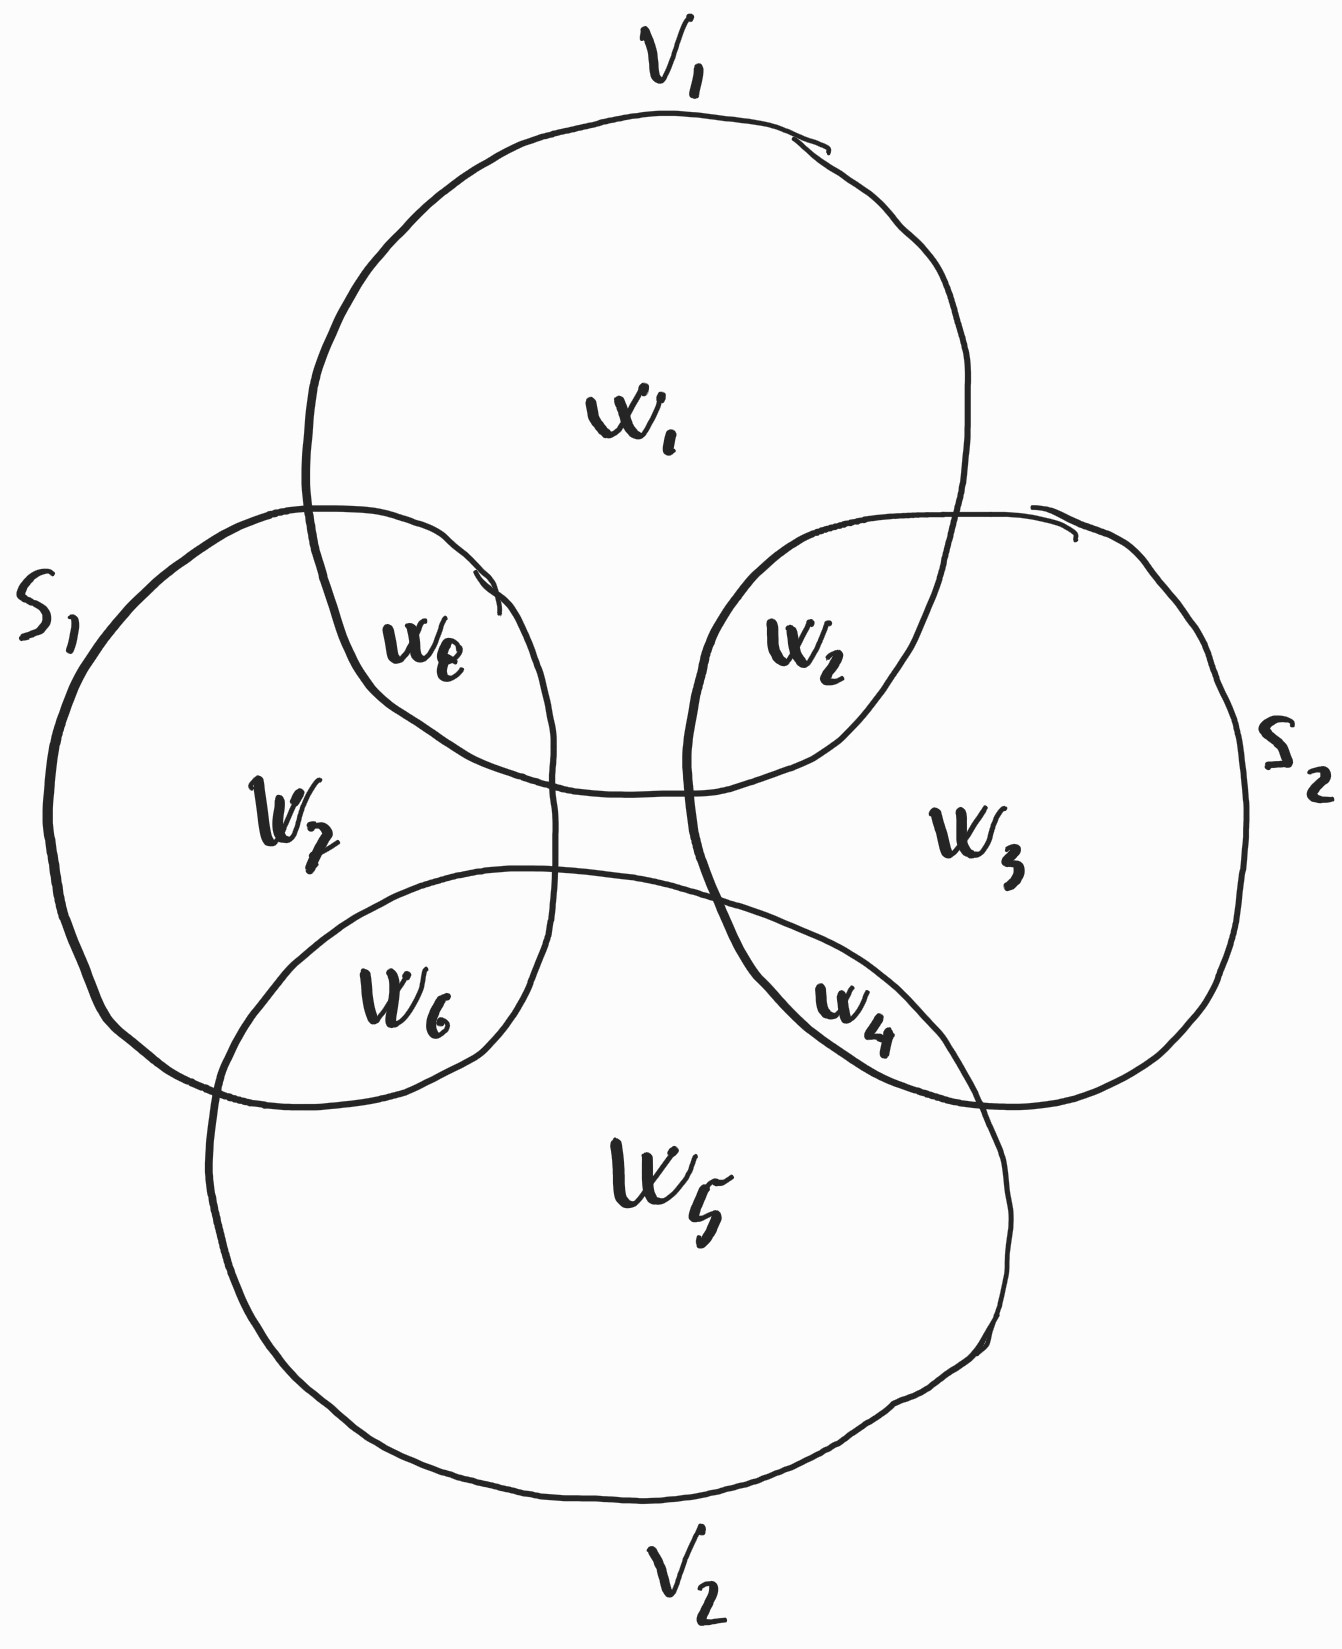
\includegraphics[scale=.2]{VillegasDiagram.jpg}
\end{center}

\begin{proof}
For 1, using the diagram as an aid, let us decompose the four statements into the disjunction of eight pairwise incompatible statements. We have
\begin{itemize}
    \item $\stmt[v]_1 \equiv \stmt[w]_1 \OR \stmt[w]_2 \OR \stmt[w]_8 $
    \item $\stmt[v]_2 \equiv \stmt[w]_4 \OR \stmt[w]_5 \OR \stmt[w]_6 $
    \item $\stmt[s]_2 \equiv \stmt[w]_2 \OR \stmt[w]_3 \OR \stmt[w]_4 $
    \item $\stmt[s]_1 \equiv \stmt[w]_6 \OR \stmt[w]_7 \OR \stmt[w]_8 $
\end{itemize}
where
\begin{itemize}
    \item $\stmt[w]_1 \equiv \stmt[v]_1 \AND \NOT \stmt[s]_1 \AND \NOT \stmt[s]_2 $
    \item $\stmt[w]_2 \equiv \stmt[v]_1 \AND \stmt[s]_2 $
    \item $\stmt[w]_3 \equiv \stmt[s]_2 \AND \NOT \stmt[v]_1 \AND \NOT \stmt[v]_2 $
    \item $\stmt[w]_4 \equiv \stmt[v]_2 \AND \stmt[s]_2 $
    \item $\stmt[w]_5 \equiv \stmt[v]_2 \AND \NOT \stmt[s]_1 \AND \NOT \stmt[s]_2 $
    \item $\stmt[w]_6 \equiv \stmt[v]_2 \AND \stmt[s]_1 $
    \item $\stmt[w]_7 \equiv \stmt[s]_1 \AND \NOT \stmt[v]_1 \AND \NOT \stmt[v]_2 $
    \item $\stmt[w]_8 \equiv \stmt[v]_1 \AND \stmt[s]_1 $
\end{itemize}

Since all $\{ \stmt[w]_i \}$ are pair-wise incompatible, offset monotonicity allows to remove or add the same statement on both sides of a fineness relationship. Therefore
\begin{itemize}
    \item $\stmt[v]_1 \coarser \stmt[s]_1 \implies  \stmt[w]_1 \OR \stmt[w]_2 \OR \stmt[w]_8 \coarser \stmt[w]_6 \OR \stmt[w]_7 \OR \stmt[w]_8 \implies \stmt[w]_1 \OR \stmt[w]_2 \coarser \stmt[w]_6 \OR \stmt[w]_7 \implies \stmt[w]_1 \OR \stmt[w]_2 \OR \stmt[w]_5 \coarser \stmt[w]_5 \OR \stmt[w]_6 \OR \stmt[w]_7$
    \item $\stmt[v]_2 \coarser \stmt[s]_2 \implies  \stmt[w]_4 \OR \stmt[w]_5 \OR \stmt[w]_6 \coarser \stmt[w]_2 \OR \stmt[w]_3 \OR \stmt[w]_4 \implies \stmt[w]_5 \OR \stmt[w]_6 \coarser \stmt[w]_2 \OR \stmt[w]_3 \implies \stmt[w]_5 \OR \stmt[w]_6 \OR \stmt[w]_7 \coarser \stmt[w]_2 \OR \stmt[w]_3 \OR \stmt[w]_7$
    \item $\stmt[w]_1 \OR \stmt[w]_2 \OR \stmt[w]_5 \coarser \stmt[w]_5 \OR \stmt[w]_6 \OR \stmt[w]_7 \coarser \stmt[w]_2 \OR \stmt[w]_3 \OR \stmt[w]_7 \implies \stmt[w]_1 \OR \stmt[w]_2 \OR \stmt[w]_5 \coarser \stmt[w]_2 \OR \stmt[w]_3 \OR \stmt[w]_7 \implies \stmt[w]_1 \OR \stmt[w]_5 \coarser \OR \stmt[w]_3 \OR \stmt[w]_7$
\end{itemize}
Finally $\stmt[w]_1 \OR \stmt[w]_5 \coarser \stmt[w]_3 \OR \stmt[w]_7 \implies \stmt[w]_1 \OR \stmt[w]_2 \OR \stmt[w]_4 \OR \stmt[w]_5 \OR \stmt[w]_6 \OR \stmt[w]_8 \coarser \stmt[w]_2 \OR \stmt[w]_3 \OR \stmt[w]_4 \OR \stmt[w]_6 \OR \stmt[w]_7 \OR \stmt[w]_8 \implies \stmt[v]_1 \OR \stmt[v]_2 \coarser \stmt[s]_1 \OR \stmt[s]_2$.

For 2, let $\hat{\stmt[s]}_2 = \stmt[s]_2 \AND \NOT \stmt[s]_1$. We have $\stmt[s]_1 \ncomp \hat{\stmt[s]}_2$ and $\hat{\stmt[s]}_2 \finer \stmt[s]_2 \finer \stmt[v]_2$ since $\hat{\stmt[s]}_2 \narrower \stmt[s]_2$. By 1, we have $\stmt[s]_1 \OR \hat{\stmt[s]}_2 \finer \stmt[v]_1 \OR \stmt[v]_2$. But since $\stmt[s]_1 \OR \hat{\stmt[s]}_2 \equiv \stmt[s]_1 \OR (\stmt[s]_2 \AND \NOT \stmt[s]_1) \equiv (\stmt[s]_1 \OR \stmt[s]_2) \AND (\stmt[s]_1 \OR \NOT \stmt[s]_1) \equiv \stmt[s]_1 \OR \stmt[s]_2$, we have $\stmt[s]_1 \OR \stmt[s]_2 \finer \stmt[v]_1 \OR \stmt[v]_2$..

\end{proof}

\begin{conj}
Other properties that show how the most you can broaden something within an equigranular equivalence class is by a disjunction with something incompatible.
	
\begin{itemize}
	\item if $\stmt_1 \ncomp \stmt_2$, $\stmt[v]_1 \ncomp \stmt[v]_2$ and $\stmt_2 \eqgran \stmt[v]_2$, then $\stmt_1 \finer \stmt[v]_1$ if and only if $\stmt_1 \OR \stmt_2 \finer \stmt[v]_1 \OR \stmt[v]_2$.
	
	\item if $\stmt[v]_1\ncomp\stmt[v]_2$, $\stmt[v]_2\eqgran\stmt_2$, and $\stmt_1\finer\stmt[v]_1$. Then $\stmt_1\OR\stmt_2\finer\stmt[v]_1\OR\stmt[v]_2$.
\end{itemize}

\end{conj}

\begin{prop}
    Equigranularity is an equivalence relationship.
\end{prop}

\begin{proof}
    It is an equivalence relationship because it is the symmetrization of a preorder. Since fineness is reflexive then equigranularity is also reflexive: for all $\stmt \in \tdomain$ $\stmt \finer \stmt$ and therefore $\stmt \eqgran \stmt$. Since fineness is transitive then equigranularity is also transitive: $\stmt_1 \eqgran \stmt_2 \eqgran \stmt_3$ means $\stmt_1 \finer \stmt_2 \finer \stmt_3$ therefore $\stmt_1 \finer \stmt_3$ but also $\stmt_3 \finer \stmt_2 \finer \stmt_1$ therefore $\stmt_3 \finer \stmt_1$ and finally $\stmt_1 \eqgran \stmt_3$. Additionally, equigranularity is reflexive by definition and is therefore an equivalence relationship.
\end{proof}

\begin{defn}
    Let $\tdomain_{/\eqgran}$ be the equivalence classes of equigranularity. We call \textbf{granularity level} an equivalence class of equigranularity. Let $(\cdot)_{/\eqgran} : \tdomain \to \tdomain_{/\eqgran}$ the map from a statement to its granularity level, which we also note $\dot{\stmt} = {\stmt}_{/\eqgran}$. We say $\dot{\stmt}$ is the granularity level of $\stmt$.
\end{defn}

\begin{prop}
    The function $(\cdot)_{/\eqgran}$ is an order homomorphism.
\end{prop}

\begin{proof}
    Let $\stmt_1, \stmt_2 \in \tdomain$. Suppose $\stmt_1 \narrower \stmt_2$ then by \ref{fineness_properties}.3 $\stmt_1 \finer \stmt_2$ and therefore ${\stmt_1}_{/\eqgran} \finer {\stmt_2}_{/\eqgran}$. Then $(\cdot)_{/\eqgran}$ is an order isomorphism.
\end{proof}

\begin{remark}
    Regardless of whether $\tdomain_{/\eqgran}$ is a lattice, $(\cdot)_{/\eqgran}$ can never be a lattice homomorphism. It will be crucial that two equigranular statements can be incompatible, and this in contradiction with $(\cdot)_{/\eqgran}$ being a lattice homomorphism. Let us note $\dot{\stmt} = {\stmt}_{/\eqgran}$ the level of granularity of $\stmt$. Now suppose that $\stmt_1 \eqgran \stmt_2 \nequiv \impossibility$ and $\stmt_1 \ncomp \stmt_2$. Then $\dot{\stmt}_1 = \dot{\stmt}_2 \neq \dot{\impossibility}$. Now suppose that $\stmt \to \dot{\stmt}$ is a lattice isomorphism. Then $\dot{\impossibility} = (\stmt_1 \AND \stmt_2)_{/\eqgran} = \dot{\stmt}_1 \wedgedot \dot{\stmt}_2 = \dot{\stmt}_1 \wedgedot \dot{\stmt}_1 = \dot{\stmt}_1$, which contradicts the premise.
\end{remark}

\begin{remark}
We claim there exist domains which have all possibilities equigranular but fineness is not a total order. Suppose we have a theoretical domain in bijection with the power set of the natural numbers, $\mathcal{P}(\mathbb{N})$. The partial order of narrowness may be given by the ordering of the power set by set containment, and the possibilities (which also serve as a countable generating set) are given by $\mathbb{N}$. The hypotheses of the fineness relation (Definition \ref{fineness}) are satisfied if we order contingent statements by cardinality, with the additional requirement that infinite strict subsets of $\mathbb{N}$ are considered strictly finer than the certainty $\mathbb{N}\in\mathcal{P}(\mathbb{N})$. All finite sets will be totally (pre)ordered, but infinite sets will not be ordered. We note that one could just say that $\stmt_1\finer\stmt_2$ for every pair of infinite contingent statements $\stmt_1,\stmt_2$, but even if we remove those from the relation $\finer$, the axioms are still satisfied, and the (pre)order is not total. 
\end{remark}

\begin{defn}
    A theoretical domain $\tdomain$ is \textbf{uniform} if fineness has the following additional properties:
    \begin{itemize}
        \item totality: for all $\stmt_1, \stmt_2 \in \tdomain$ either $\stmt_1 \finer \stmt_2$ or $\stmt_2 \finer \stmt_1$
        \item uniformity: all possibilities are equigranular.
    \end{itemize}

\end{defn}

\begin{prop}
	Let $\tdomain$ be a theoretical domain. If all possibilities are equigranular, then the fineness class of statements compatible with only finitely many possibilities is determined by the number of possibilities with which they are compatible.
\end{prop}
\begin{proof}
	Assume all possibilities are equigranular and let $\stmt_1$ and $\stmt_2$ be compatible with finitely many possibilities. We show that if $\stmt_1$ is compatible with at least as many possibilities as $\stmt_2$, then $\stmt_2\finer\stmt_1$. We proceed by induction on $N$, the number of possibilities compatible with $\stmt_1$. The case of $N=1$ follows from equigranularity of possibilities. Now suppose the claim holds for some $N$. Let $\stmt_1 = p_1\OR\cdots\OR p_{N+1}$ and $\stmt_2 = q_1\OR\cdots\OR q_m$ be statements compatible with only finitely many possibilities $p_i,i=1,\ldots,N+1$ and $q_j,j=1,\ldots,m$ respectively, where $m\leq N+1$. 
	
	Consider first the case where $m\leq N$. Then $\stmt_2 \finer p_1\OR\cdots\OR p_N \sfiner p_1\OR\cdots\OR p_N\OR p_{N+1} = \stmt_1$, so $\stmt_2\finer\stmt_1$. Next, suppose $m=N+1$. Write $\stmt_1' = p_1\OR\cdots\OR p_N$ and $\stmt_2' = q_1\OR\cdots\OR q_N$. We have already that all disjunctions of $N$ possibilties are equigranular, so $\stmt_1'\eqgran\stmt_2'$. Possibly by rearranging the order of the possibilties in the disjunction, we may assume $q_{N+1}\ncomp\stmt_1'$ and $q_{N+1}\ncomp\stmt_2'$. By Proposition \ref{fineness_properties}, we have $\stmt_1\OR q_{N+1}\eqgran\stmt_2$. Similarly, since $p_{N+1}\eqgran q_{N+1}$, we have $\stmt_1\eqgran\stmt_1'\OR q_{N+1}$. We conclude that $\stmt_1\eqgran\stmt_2$. 
\end{proof}


\begin{coro}
	Let $\tdomain$ be such that all possibilities are equigranular. Let $x \in \tdomain$ be a possibility. Then there exists a unique measure $\mu_{x} : \tdomain \to \mathbb{R} \cup \{+\infty\}$ which corresponds to the counting measure of possibilities compatible to the statement.
\end{coro}

We expect the following to not be provable from the given axioms:

\begin{desid}\label{uniformconsequence}
    Let $\tdomain$ be uniform. Let $\stmt, \stmt_1 \in \tdomain$ such that $\stmt \sfiner \stmt_1$. Then there exist $\stmt_2 \in \tdomain$ such that $\stmt_2 \narrower \stmt_1$ and $\stmt \eqgran \stmt_2$.
\end{desid}
However, it would be nice to understand why as it would give us insights into which additional premises are needed. The idea is that we can always ``move" a statement to an equigranular one to sit within any other (coarser) statement. This would allow us to make use of various properties of narrowness. Interestingly, this would not give additional insight into limiting behaviors, as equigranular sequences may have vastly different limits (and so ``moving" a sequence could drastically change the equigranularity class of the limit).

\subsection{Infinitesimals}

The following is an attempt to define infinitesimal in a way that puts the least constraints on fineness.

\begin{defn}\label{infinitesimals}
	Let $\stmt[u],\stmt[s] \in \tdomain$. Then $\stmt$ is \textbf{infinitesimal} with respect to $\stmt[u]$ if for any natural number $n$ we can find a set of $n$ statements $\{ \stmt_i \}_{i=1}^n$ such that:
	\begin{enumerate}
		\item $\stmt \finer \stmt_i$ for all $i$
		\item $\stmt_i \ncomp \stmt_j$ for all $i \neq j$
		\item $\bigOR\limits_{i=1}^n \stmt_i \finer \stmt[u]$ 
	\end{enumerate}
	In words, $\stmt$ is infinitesimal with respect to $\stmt[u]$ if for any number, there is a disjunction of that many broader mutually incompatible statements $\stmt_i$ is finer than $\stmt[u]$.
\end{defn}

\begin{remark}
	Note that we do not require the $\stmt_i$ to be equigranular to $\stmt$. Also note that, with this definition, a statement can fail to be infinitesimal simply because one cannot find enough statements comparable to both $\stmt$ and $\stmt[u]$.
\end{remark}

\begin{coro}
	The impossibility $\impossibility$ is an infinitesimal with respect to any $\stmt[u] \in \tdomain$.
\end{coro}

\begin{proof}
	Let $\stmt[u] \in \tdomain$ and consider $\{ \stmt_i \}_{i=1}^n$ where $\stmt_i \equiv \impossibility$ for all $i$. Then $\impossibility \finer \impossibility \equiv \stmt_i$ for all $i$. Since $\impossibility \ncomp \impossibility$, $\stmt_i \ncomp \stmt_j$ for all $i$ and $j$. Lastly, $\bigOR\limits_{i=1}^n \stmt_i \equiv \impossibility \finer \stmt[u]$. This means that $\{ \stmt_i \}_{i=1}^n$ realizes infinitesimality for $\impossibility$, which is an infinitesimal of $\stmt[u]$.
\end{proof}

\begin{defn}
	Let $\stmt, \stmt[u] \in \tdomain$ be two statements such that $\stmt \finer \stmt[u]$. We say that they are \textbf{finitely comparable} to each other if we can find a finite set $\{ \stmt_i \}_{i=1}^n$ such that $\stmt_i \finer \stmt$ for all $i \leq n$ and $\stmt[u] \finer \bigOR_{i=1}^n \stmt_i$.
\end{defn}

TODO[Mark]: check the proof
\begin{prop}
	If two statements are finitely comparable then they cannot be infinitesimals with respect to each other.
\end{prop}
\begin{proof}
	Suppose $\stmt$ and $\stmt[u]$ are finitely comparable. Then we can find a set of $n$ statements $\{ \stmt_i \}_{i=1}^n$ such that $\stmt_i \finer \stmt$ for all $i \leq n$ and $\stmt[u] \finer \bigOR_{i=1}^n \stmt_i$. Now suppose we have a set of statements $\{ \stmt[t]_i \}_{i=1}^n$ such that $\stmt \finer \stmt[t]_i$ for all $i$ and $\stmt[t]_i \ncomp \stmt[t]_j$ for all $i \neq j$. Then we also have $\stmt_i \finer \stmt \finer \stmt[t]_i$ for all $i$. By \ref{fineness_monotony} we have $\bigOR_{i=1}^n \stmt_i \finer \bigOR_{i=1}^n \stmt[t]_i$ and therefore $\stmt[u] \finer \bigOR_{i=1}^n \stmt_i \finer \bigOR_{i=1}^n \stmt[t]_i$. Therefore we cannot find a set of $n$ statement that satisfy the definition of infinitesimal and therefore $\stmt$ is not an infinitesimal with respect to $\stmt[u]$.
\end{proof} 

\begin{prop}\label{infinitesimal_conjunction}
	Let $\stmt \in \tdomain$ be an infinitesimal with respect to $\stmt[u] \in \tdomain$. Then any $\stmt[v] \finer \stmt$ is also an infinitesimal with respect to $\stmt[u]$.
\end{prop}
\begin{proof}
	Since $\stmt$ is an infinitesimal with respect to $\stmt[u]$, for any $n$ we can find a set of statements $\{ \stmt_i \}_{i=1}^n$ that realizes its infinitesimality. We have $\stmt[v] \finer \stmt \finer \stmt_i$ for all $i$. The other two properties do not depend on $\stmt$. Therefore $\{ \stmt_i \}_{i=1}^n$ realizes infinitesimality for $\stmt[v]$ as well so $\stmt[v]$ is an infinitesimal with respect to $\stmt[u]$.
\end{proof}

\begin{coro}
	The conjunction of two infinitesimals with respect to $\stmt[u]$ is infinitesimal with respect to $\stmt[u]$.
\end{coro}
\begin{proof}
	Let $\stmt[v]_1, \stmt[v]_2 \in \tdomain$ be infinitesimal with respect to $\stmt[u]$. Since $\stmt[v]_1 \AND \stmt[v]_2 \narrower \stmt[v]_1$, $\stmt[v]_1 \AND \stmt[v]_2 \finer \stmt[v]_1$ and therefore $\stmt[v]_1 \AND \stmt[v]_2$ by \ref{infinitesimal_conjunction}.
\end{proof}

\begin{prop}\label{infinitesimal_disjunction}
	The disjunction of two infinitesimals with respect to $\stmt[u]$ that are comparable\footnote{Is comparability required? Can it be proved one way or another?} to each other is infinitesimal with respect to $\stmt[u]$.
\end{prop}
\begin{proof}
	Let $\stmt[v],\stmt[w]$ be infinitesimal with respect to $\stmt[u]$. Without loss of generality, suppose $\stmt[v] \finer \stmt[w]$. Let $n>0$. Let $\{\stmt[w]_i\}_{i=1}^{2n}$ be a collection realizing infinitesimality for $2n$ for $\stmt[w]$. Define $\stmt_j = \stmt[w]_j\OR\stmt[w]_{j+n}$ for $j=1,\ldots,n$. Notice that the $\stmt_j$'s are mutually incompatible, and their disjunction must be finer than $\stmt[u]$. Further, since $\stmt[v]\finer\stmt[w]$ we have that $\stmt[v]\finer\stmt[w]_i$ for all $i$. It follows that:
	$$
	\stmt[v]\OR\stmt[w] \finer \stmt[w]_j\OR\stmt[w]_{j+n} = \stmt_j
	$$
	for all $j=1,\ldots,n$. Thus the collection $\{\stmt_j\}_{j=1}^n$ realizes $\stmt[v]\OR\stmt[w]$ being infinitesimal with respect to $\stmt[u]$ for $n$. We conclude that $\stmt[v]\OR\stmt[w]$ is infinitesimal with respect to $\stmt[u]$. 
\end{proof}

\begin{prop}[Infinitesimality is consistent with fineness]\label{infinitesimal_finess}
	Let $\stmt[u],\stmt[v]$ be statements such that $\stmt[v]\finer\stmt[u]$. Let $\stmt$ be an infinitesimal with respect to $\stmt[v]$. Then $\stmt$ is infinitesimal with respect to $\stmt[u]$. 
\end{prop}
\begin{proof}
	Let $n>0$ be a natural number, and let $\{ \stmt_i \}_{i=1}^n$ be as in the definition of infinitesimal for $\stmt$ with respect to $\stmt[v]$. Then $\{ \stmt_i \}_{i=1}^n$ also satisfies the requirements for infinitesimal with respect to $\stmt[u]$. The first two requirements are unchanged, and the third is easy to see:
	$$
	\bigOR\limits_{i=1}^n \stmt_i \finer\stmt[v]\finer \stmt[u]
	$$
\end{proof}

\begin{coro}[Infinitesimality is consistent with narrowness]
	Let $\stmt[u],\stmt[v]$ be statements such that $\stmt[v]\narrower\stmt[u]$. Let $\stmt$ be an infinitesimal with respect to $\stmt[v]$. Then $\stmt$ is infinitesimal with respect to $\stmt[u]$.
\end{coro}
\begin{proof}
	Since $\stmt[v]\narrower\stmt[u]$ implies $\stmt[v]\finer\stmt[u]$, proposition \ref{infinitesimal_finess} applies.
\end{proof}

We wish to also show some form of compatibility in the reverse direction. That is, if we shrink by a ``finite" amount, the sets which were previously infinitesimal should remain so (of course, if we shrink by an ``infinite" amount, e.g. by dropping a dimension, previously infinitesimal sets may no longer be so). 

\begin{prop}
	Let $\tdomain$ be uniform. Let $\stmt[u],\stmt[v] \in \tdomain$ be statements such that $\stmt[v]$ is not infinitesimal with respect to $\stmt[u]$. Let $\stmt$ be a statement $\stmt\narrower\stmt[v]$ such that $\stmt$ is infinitesimal with respect to $\stmt[u]$. Then $\stmt$ is infinitesimal with respect to $\stmt[v]$. 
\end{prop}
\begin{proof}
	Note: the use of totality is highlighted as we would like to, if possible, remove it.
	
	Let $\stmt[u]$, $\stmt[v]$, and $\stmt$ be as in the Proposition statement. We will show that $\stmt$ is infinitesimal with respect to $\stmt[v]$. To do so, we will show that for any $n>0$, we can find a set of $n$ statements $\{\stmt_i\}_{i=1}^n$ such that: 
	\begin{enumerate}
		\item $\stmt \finer \stmt_i$ for all $i$
		\item $\stmt_i \ncomp \stmt_j$ for all $i \neq j$
		\item $\bigOR\limits_{i=1}^n \stmt_i \finer \stmt[v]$ 
	\end{enumerate}
	We will show this for arbitrary $n$, which will be sufficient to prove that $\stmt$ is infinitesimal with respect to $\stmt[v]$. 
	
	First, since $\stmt[v]$ is not infinitesimal with respect to $\stmt[u]$, there exists some $N>0$ such that for any set of $N$ statements, at least one of the conditions of infinitesimality of $\stmt[v]$ with respect to $\stmt[u]$ fails. 
	
	Let $n>0$. Let $\{\stmt_i\}_{i=1}^{nN}$ be a set of $n\cdot N$ statements realizing infinitesimality of $\stmt$ with respect to $\stmt[u]$ (i.e. they are mutually incompatible, broader than $\stmt$, and their disjunction is narrower than $\stmt[u]$). 
	
	{\bf By totality of $\finer$}\footnote{What we needed here is that there is a partition of the collection into $N$ sets of size $n$ such that for one of them, their disjunction is finer than each of $N-1$ disjunctions of the other subsets in the partition.}, we may assume the collection $\{\stmt_i\}_{i=1}^{nN}$ is ordered by fineness ($\stmt_1\finer\stmt_2\finer\cdots$). Consider the finest $n$ statements, that is, consider the collection $\{\stmt_i\}_{i=1}^{n}$. We will show that this collection satisfies the conditions for $\stmt$ being infinitesimal with respect to $\stmt[v]$ for $n$ statements. 
	
	By construction, this satisfies properties 1 and 2 for infinitesimality of $\stmt$ in $\stmt[v]$, since it is a subset of a collection which already satisfied those properties. 
	
	Now suppose it fails property 3\footnote{We will use totality since we need $\NOT \big(\stmt[x]\sfiner\stmt[y]\big) \implies \stmt[x]\coarser\stmt[y]$.}, that is, suppose 
	$$
	\bigOR\limits_{i=1}^n \stmt_i \scoarser\stmt[v].
	$$
	We will show that this will lead to a contradiction by implying that there is a collection of statements of size $N$ realizing $\stmt[v]$ being infinitesimal with respect to $\stmt[u]$. 
	
	Consider now the collection of $N$ statements $\{\stmt[a]_j\}_{j=1}^N$ defined by $$\stmt[a]_j = \bigOR\limits_{i=n(j-1)+1}^{nj}\stmt_i.$$
	These statements are built from the collection $\{\stmt_i\}_{i=1}^{n}$ by taking $N$ disjunctions each consisting of $n$ of the statements. Notice that $\stmt[a]_1$ is the disjunction of the collection $\{\stmt_i\}_{i=1}^{n}$ considered above. 
	
	First, this collection is mutually incompatible, since it is made up of disjunctions of mutually incompatible statements. This is property 2 for $\stmt[v]$ being infinitesimal with respect to $\stmt[u]$. 
	
	Next, these must satisfy property 1 for $\stmt[v]$ being infinitesimal with respect to $\stmt[u]$. To see why, notice that by our assumption, we have $\stmt[a]_1\scoarser\stmt[v]$, and by construction, we have $\stmt[a]_j\coarser\stmt[a]_1$ for all $j=1,\ldots,N$, and so $\stmt[v]\finer\stmt[a]_j$ for all $j=1,\ldots,N$. 
	
	Finally, they also must satisfy property 3: $$\stmt[a]_1\OR\cdots\OR\stmt[a]_N = \bigOR\limits_{i=1}^{nN}\stmt_i\finer\stmt[u].$$
	
	Thus, this new collection violates the assumption that no set of $N$ statements satisfies all three properties for $\stmt[v]$ being infinitesimal in $\stmt[u]$. 
	
	{\bf By totality of $\finer$},\footnote{Here we are using totality as specified in the previous footnote.} we conclude that we must have $\bigOR\limits_{i=1}^n \stmt_i \finer\stmt[v]$ as required, and so the collection $\{\stmt_i\}_{i=1}^{n}$ realizes $\stmt$ being infinitesimal with respect to $\stmt[v]$ for $n$ statements. Since $n$ was arbitrary, it must be the case that $\stmt$ is infinitesimal with respect to $\stmt[v]$. 
\end{proof}

\subsection{Comparision and equivalence at $\stmt[u]$ scale}

The general idea is to collapse the preorder given by fineness $\finer$ so that statements that are different up to an infinitesimal are equal.

\def\equivu{\cong_{\stmt[u]}}

\begin{defn}
	Let $\stmt_1, \stmt_2 \in \tdomain$. We say $\stmt_1$ is \textbf{equivalent to $\stmt_2$ at $\stmt[u]$ scale}, noted $\stmt_1 \equ \stmt_2$, if we can find $\stmt[v]_1, \stmt[v]_2 \in \tdomain$ that are infinitesimal with respect to $\stmt[u]$ such that $\stmt_1 \OR \stmt[v]_1 \eqgran \stmt_2 \OR \stmt[v]_2$.
\end{defn}

When the definitions and axioms are solidified, the following will be essential: 

\begin{desid}
	Equivalence at $\stmt[u]$ scale is an equivalence relation.
\end{desid}

\begin{remark}
	For reflexivity, let $\stmt \in \tdomain$. We have $\stmt \OR \impossibility \equiv \stmt \OR \impossibility$. Since $\impossibility$ is an infinitesimal for all $\stmt[u]$, $\stmt \equ \stmt$. For symmetry, note that the definition itself is symmetrical.
	
	Transitivity is unclear. Let $\stmt_1 \equ \stmt_2 \equ \stmt_3$. Then we can write $\stmt_1 \OR \stmt[v]_1 \eqgran \stmt_2 \OR \stmt[v]_2$ and $\stmt_2 \OR \stmt[w]_2 \eqgran \stmt_3 \OR \stmt[w]_3$. If the infinitesimal where incompatible we would have $\stmt_1 \OR \stmt[v]_1 \OR \stmt[w]_2 \eqgran \stmt_2 \OR \stmt[v]_2 \OR \stmt[w]_2 \eqgran \stmt_3 \OR \stmt[w]_3 \OR \stmt[v]_2$. If the infinitesimals were comparable, by proposition \ref{infinitesimal_disjunction} we would have that $\stmt[v]_1 \OR \stmt[w]_2$ and $\stmt[w]_3 \OR \stmt[v]_2$ are infinitesimals and therefore $\stmt_1 \equ \stmt_3$.
	
	If we assume a uniform domain, we would have totality and we may also be able to show that incompatible infinitesimals can always be found. It may be that totality is not needed for proposition \ref{infinitesimal_disjunction}. It may be that we need to amend the definition of infinitesimals, such that the disjunction of two infinitesimals is an infinitesimals. We could also force the transitivity, even if the disjunction of two infinitesimals is not an infinitesimals. This would be like saying that, yes, in principles the assertions correspond to different granularity levels, but we are not to distinguish between them because the different is effectively zero. Understanding which options are best requires more work.
\end{remark}

Another essential property of equivalence at $\stmt[u]$ scale is that it collapses the fineness ordering, formalized by the following statement:

\begin{desid}
	Let $\stmt_1, \stmt_2 \in \tdomain$ such that $\stmt_1 \equ \stmt_2$ and $\stmt_1 \finer \stmt_2$. Then for all $\stmt_1 \finer \stmt \finer \stmt_2$ we have $\stmt_1 \equ \stmt \equ \stmt_2$.
\end{desid}

\begin{remark}
	What we'd like to have is that equivalence at $\stmt[u]$ scale merges contiguous granularity levels. It is yet to be understood what are the necessary preconditions for which this happens. One conjecture is that a uniform domain would be sufficient, though probably not necessary.
\end{remark}

A special case of the above may be a good first goal for testing appropriate axioms, or perhaps it could end up being an axiom itself:

\begin{desid}
	Let $\stmt_1,\stmt,\stmt[v]_1\in\tdomain$ such that $\stmt_1\finer\stmt\finer\stmt_1\OR\stmt[v]_1$, and suppose $\stmt[v]_1$ is infinitesimal with respect to $\stmt[u]$. Then $\stmt\equ\stmt_1$. 
\end{desid}

In addition to defining equivalence at scale $\stmt[u]$, we also wish to have the ordering. Eventually, the goal is to use this as a qualitative probability, as in Fishburn \cite{fishburnsurvey}. 

\begin{defn}\label{smalleru}
	Let $\stmt_1, \stmt_2 \in \tdomain$. Then $\stmt_1$ is \textbf{smaller than} $\stmt_2$ \textbf{in} $\stmt[u]$, noted $\stmt_1 \lequ \stmt_2$, if $\stmt_1 \finer \stmt_2$ or $\stmt_1 \equ \stmt_2$. We define $\stmt_1\ltu\stmt_2$ by $\stmt_1\lequ\stmt_2$ and not $\stmt_1\equ\stmt_2$. 
\end{defn}

This is the final notion of ordering. After narrowness orders the actual content of the statements and fineness gives a very precise ordering of size, ordering by scale in $\stmt[u]$ aims to give a less universal notion of size relative to a fixed unit statement $\stmt[u]$, where we collapse by equivalence at scale. 

An alternative definition is as follows. 

\begin{defn}\label{smalleru2}
	Let $\stmt_1, \stmt_2 \in \tdomain$. Then $\stmt_1$ is \textbf{smaller than} $\stmt_2$ \textbf{in} $\stmt[u]$, noted $\stmt_1 \lequ \stmt_2$, if there exist statements $\stmt_1'$ and $\stmt_2'$ with $\stmt_1'\equ\stmt_1$ and $\stmt_2'\equ\stmt_2$ such that $\stmt_1'\finer\stmt_2'$.
\end{defn}

We still need to show the following:

\begin{desid}
	The two definitions are equivalent.
\end{desid}

\begin{remark}
	The idea is that smallness in $\stmt[u]$ compares the equivalence classes at $\stmt[u]$ scale. In other words, we should be able to show that the map $\tdomain / \eqgran \to \tdomain / \equ$ defined by collapsing equivalence classes is well-defined and monotonic. There may be a more natural order theoretic definition that automatically does this, and shows that smallness in $\stmt[u]$ is a preorder.
\end{remark}

The following property is crucial for the theory of qualitative probability, but fortunately it is immediate from either definition. 

\begin{prop}
For all statements $\stmt$ and $\stmt[u]$, we have $\impossibility\lequ\stmt\lequ\certainty$.
\end{prop}
\begin{proof}
	Since $\impossibility \finer \stmt$ for any $\stmt$, we have $\impossibility\lequ\stmt$ regardless of the choice of $\stmt[u]$. Conversely, since $\stmt \finer \certainty$ for any $\stmt$, we have $\stmt\lequ\certainty$ regardless of the choice of $\stmt[u]$.
\end{proof}

\begin{prop}
	If for every statement $\stmt[v]$ infinitesimal in $\stmt[u]$, we have $\stmt_1\OR\stmt[v] \sfiner \stmt_2$, then we have $\stmt_1 \ltu \stmt_2$. 
\end{prop}
\begin{proof}
	First, using $\stmt[v] = \impossibility$ (an infinitesimal) in the hypothesis of the statement, we have $\stmt_1 = \stmt_1\OR\impossibility \sfiner \stmt_2$, and so by Definition \ref{smalleru}, we have that $\stmt_1\lequ\stmt_2$. Now, we must show it is not the case that $\stmt_1\equ \stmt_2$. 
	
	Suppose that $\stmt_1 \equ \stmt_2$. By Definition \ref{smalleru}, let $\stmt[v]_1,\stmt[v]_2\in\tdomain$ be infinitesimals such that $\stmt_1 \OR \stmt[v]_1 \eqgran \stmt_2 \OR \stmt[v]_2$. But by assumption, $\stmt_1\OR\stmt[v]_1 \sfiner \stmt_2 \finer\stmt_2\OR\stmt[v]_2$. This contradicts the earlier equigranularity, and so it cannot be the case that $\stmt_1\equ\stmt_2$. 
\end{proof}

We need it to be the case that $\lequ$ is a pre-order, and that it is a partial order with respect to $\equ$-equivalence classes. 

\begin{desid}
	The relation $\lequ$ is reflexive and transitive and therefore a preorder. 
\end{desid}

Fortunately, at least the first definitions of $\lequ$ and $\equ$ behave well together:

\begin{prop}
	If $\stmt_1\lequ\stmt_2$ and $\stmt_1\gequ \stmt_2$, then $\stmt_1\equ\stmt_2$.
\end{prop}
\begin{proof}
	This is immediate from the first definition, since we would either have $\stmt_1\eqgran\stmt_2$ (which implies $\stmt_1\equ\stmt_2$), or we would already have $\stmt_1\equ\stmt_2$.
\end{proof}

For the second definition of $\lequ$, transitivity of $\equ$ is needed which we have not proven. 

Question: is the map $\tdomain / \eqgran \to \tdomain / \equ$ defined by collapsing equivalence classes well-defined and monotone? 

Eventually, we wish to use $\lequ$ as a total pre-order in order to use it as a qualitative probability. We will need an interesting-enough subset of $\tdomain$ to capture the desired notions while still having $\lequ$ as a total order.

\subsubsection{Collapsing Orders}
In Section 2.1 of \cite{quotientposets}, the idea of collapsing a poset by an equivalence relation is introduced. 

If $(P,\leq)$ is a poset and $\sim$ is a collapsing equivalence relation, we may endow the set $P_{/\sim}$ with the relation $\leq_{/\sim}$ defined by $x_{/\sim} \leq_{/\sim} y_{/\sim}$ whenever there exist $x'\in x_{/\sim}$ and $y'\in y_{/\sim}$ with $x'\leq y'$ (this is the definition used in \cite{quotientposets}). 

It turns out that $(P_{/\sim},\leq_{/\sim})$ is not always a poset. Here is an important example. Let our set be $\{w,x,y,z\}$ and a poset relation defined by $x\leq w$, $y\leq w$, $y\leq z$, with the following Hasse diagram:

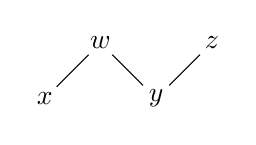
\begin{tikzpicture}
% First, locate each of the nodes and name them
\node (top) at (0,0) {$w$};
\node [below left  of=top] (left)  {$x$};
\node [below right of=top] (bottom right) {$y$};
\node [above right of=bottom right] (right) {$z$};

% Now draw the lines:
\draw [shorten <=-2pt, shorten >=-2pt] (top) -- (left);
\draw [shorten <=-2pt, shorten >=-2pt] (top) -- (bottom right);
\draw [shorten <=-2pt, shorten >=-2pt] (bottom right) -- (right);
\end{tikzpicture}

Let's consider two possible cases. Suppose first $w\sim y$, and $x$ and $z$ are only $\sim$ with themselves. Then in order to collapse $\leq$ under $\sim$, we will need $x \leq w\sim y \leq z$ for transitivity. 

Consider next the case that $w\sim y$ and $x\sim z$. In order to collapse this, we will need that $w\sim x\sim y \sim z$.

These examples show that not every equivalence relation can collapse a poset into a poset (even if it only collapses a chain). 

Lemma 2.1.3 in \cite{quotientposets} gives sufficient conditions on the interaction of $\leq$ and $\sim$ on $P$ for $(P_{/\sim},\leq_{/\sim})$ to be a poset. These essentially prevent problems of the above form from happening. 

\begin{prop}
Suppose $(P,\leq)$ has a minimum element $m$ and that the equivalence class $m_{/\sim}$ contains no other elements. Further, suppose that if $x_{/\sim} \leq_{/\sim} y_{/\sim}$, then for all $x'\in x_{/\sim}$ there exists a $y'\in y_{/\sim}$ with $x'\leq y'$. 
Under these assumptions, $(P_{/\sim},\leq_{/\sim})$ is also a poset.
\end{prop}

As for a minimum element, we have the impossibility $\impossibility$ which will be unique in its equigranularity class, but being infinitesimal it will share its $\equ$ equivalence class, so perhaps modification of the above lemma will be necessary. 

\subsection{Monotone continuity up to infinitesimals}

The established results in the literature of comparable probability require a specific axiom, called monotone continuity, that essentially make sure that sequences converge. This is necessary because their goal is to recover a probability measure that is countably additive.

\begin{defn}[Monotone continuity]\label{monotone_continuity}
	Given a domain $\tdomain$ and a unit $\stmt[u] \in\tdomain$, we say that $\lequ$ satisfies \textbf{monotone continuity} if the following is true: given a sequence $\{\stmt_i\}_{i=1}^{\infty}$ such that $\stmt_i \narrower \stmt_j$ for all $ i \leq j$ and $\stmt = \bigOR_i\stmt_i$ the disjunction, for every $\stmt[t] \in \tdomain$ such that $\stmt_i\leq_{\stmt[u]} \stmt[t]$ for all $i$ we have $\stmt\leq_{\stmt[u]} \stmt[t]$.
\end{defn}

Note that, in general, monotone continuity is not satisfied. See examples in \ref{lack_of_monotone_continuity}. In terms of measures, the issue is that we may have that the disjoint disjuntion of countably many infinitesimals is not necessarily an infinitesimal, which means countably meany sets of measure zero would not sum up to a set of measure zero.

We therefore want to make the following distinction.

\begin{defn}
We say that $\stmt$ is a \textbf{countable infinitesimal} with respect to $\stmt[u]$ if it satisfies the following conditions:
\begin{enumerate}
    \item $\stmt$ is an infinitesimal with respect to $\stmt[u]$
    \item there exists a (countable) sequence $\{\stmt_i\}_{i=1}^{\infty}$ such that $\stmt_i\finer\stmt$ for all $i$, and $\bigOR\limits_{i=1}^{\infty}\stmt_i$ is comparable but not infinitesimal with respect to $\stmt[u]$
\end{enumerate}
An infinitesimal which is not a countable infinitesimal will be called an \textbf{uncountable infinitesimal}. 
\end{defn}


An example of a space with countable infinitesimals is the natural numbers $\mathbb{N}$. If the possibilities are natural numbers themselves and they are equigranular, for any infinite subset $S$ of $\mathbb{N}$, each natural number is infinitesimal with respect to $S$. However, a countable sequence of natural numbers may not be infinitesimal with respect to $S$ (and indeed may surpass $S$ in coarseness). Another example of countable infinitesimals is any subset of $\mathbb{R}$ of finite positive Lebesgue measure. 

An example of a space with no countable infinitesimals with respect to the full space is an interval of finite length in $\mathbb{R}$ (any positive-Lebesgue measure subset will work). To see why, note that all infinitesimals are measure zero, and any countable union of measure zero sets is still measure zero. 

It seems possible that the only obstruction to monotone continuity is countable infinitesimals, since they allow limits of equigranular sequences to be of different granularity classes. 

\begin{desid}
    If $\stmt[u]$ is such that there are no countable infinitesimals, then $\lequ$ has monotone continuity. 
\end{desid}

A hint in that direction is given by the following proposition, given with no proof by \cite{villegas}.

\begin{prop}
	A necessary and sufficient condition for $\lequ$ to be monotonely continuous is the following. Let  $\{\stmt_i\}_{i=1}^{\infty}$ be a monotone sequence, that is $\stmt_i \narrower \stmt_j$ for all $i \leq j$ and $\stmt = \bigOR_i\stmt_i$ the disjunction, and let $\stmt[t] \in \tdomain$ such that $\stmt[t] \ltu \stmt$, then there exists an $n > 0$ such that $\stmt[t] \ltu \stmt_n$.
\end{prop}

Before achieving the above, it may be possible to obtain a related result about fineness and monotone continuity, which could translate to monotone continuity for $\lequ$. 

\begin{desid}
Let $\stmt[u]$ be a statement which does not admit countable infinitesimals, and let $\{\stmt_i\}_{i=1}^{\infty}$ be a sequence of statements monotone increasing in narrowness (i.e. $\stmt_i\narrower\stmt_j$ for all $i\leq j$). Write $\stmt=\OR_i\stmt_i$ for the disjunction and assume $\stmt$ is finitely comparable to $\stmt[u]$. If $\stmt[t]\in\tdomain$ such that $\stmt[t]$ is finitely comparable to $\stmt[u]$, and $\stmt_i\finer\stmt[t]$ for all $i$, then $\stmt\finer\stmt[t]\OR\stmt[w]$ for some infinitesimal (with respect to $\stmt[u]$) $\stmt[w]$. 
\end{desid}

\section{Adapting results from \cite{villegas}}

The paper \cite{villegas} by Villegas gives us some conditions under which we can recover a probability measure given a preorder. Here we state the conditions required in terms of $\lequ$ and $\tdomain_{\stmt[u]}$, which we take it to be the set of statements narrower than $\stmt[u]$. We start from the axioms of pre-order:

\begin{itemize}
	\item Totality: If $\stmt_1,\stmt_2\in \tdomain_{\stmt[u]}$, then $\stmt_1 \lequ \stmt_2$ or $\stmt_2 \lequ \stmt_1$
	\item Reflexivity: For all statements $\stmt\in \tdomain_{\stmt[u]}$, we have $\stmt\lequ\stmt$
	\item Transitivity: For all statements $\stmt_1,\stmt_2,\stmt_3\in \tdomain_{\stmt[u]}$, if $\stmt_1\lequ\stmt_2$ and $\stmt_2\lequ\stmt_3$, then $\stmt_1\lequ\stmt_3$.
	\item Boundedness: We have $\impossibility\ltu\certainty$. For all $\stmt\in \tdomain_{\stmt[u]}$ we have $\impossibility\leq_{\stmt[u]}\stmt\lequ\certainty$
\end{itemize}

Next is the axiom of monotony. Let $\stmt_1,\stmt_2,\stmt[t]_1,\stmt[t]_2 \in \tdomain_{\stmt[u]}$ with $\stmt[t]_1 \ncomp \stmt[t]_2$. Then from $\stmt_1 \lequ \stmt[t]_1$ and $\stmt_2 \lequ \stmt[t]_2$ if follows that $\stmt_1\OR \stmt_2 \lequ \stmt[t]_1\OR \stmt[t]_2$. Moreover, if $\lequ$ is replace by $\ltu$ in one of the first two equality, then the last one holds with $\ltu$.

Apart from totality, we have similar properties already defined on fineness. We will need to understand on what conditions they can be carried to $\lequ$. The best way forward will be to assume totality and see whether the other properties can be derived at least in that case.

Next we have the axiom of monotone continuity (Definition \ref{monotone_continuity}). This we have seen before and we suspect is connected to the lack of countable infinitesimals.

The last condition is the lack of atoms. An atom is defined in the following way:

\begin{defn}
An \textbf{atom} is a statement $\stmt\in S$ such that $\impossibility \ltu \stmt$ and there does not exist any statement $\stmt_2\in S$ such that $\impossibility \ltu \stmt_2 \ltu \stmt$. 
\end{defn}

Essentially, an atom is an immediate successor of the impossibility. In our framework, the possibilities are the immediate successor of the impossibility under narrowness and fineness. If the unit contains finitely many possibilities, then we will have atoms for $\lequ$. However, in that case we will assume equigranular possibilities, and therefore the counting measure will apply. If the unit has infinitely many possibilities and the possibilities are equigranular, then all possibilities are infinitesimals. We should be able to show that, in that case, there are no atoms.

The presence or lack of atoms has several important consequences. In particular, Theorem 5 in \cite{villegas} \S3 includes the fact that $\tdomain_{\stmt[u]}$ is atomless if and only if every statement can be partitioned into two equiprobable statements. Theorem 3 in \S4 states that if $\tdomain_{\stmt[u]}$ is atomless, then there exists a unique probability measure compatible with $\leq_{\stmt[u]}$, and it is countably additive. 

A major goal of this work is to discover the right axioms and definitions that will lead to a notion of $\lequ$ which has the properties necessary for the existence (and uniqueness) of a compatible probability measure on $\tdomain_{\stmt[u]}$. The above axioms discussed are enough - several theorems from \cite{villegas} give the desired result (in particular, see Theorem 3 in Section 4 and Theorem 5(iv) in Section 3, as well as their proofs). However, we have not as of yet been able to prove that $\lequ$ has the right properties. It is also possible that our framework will allow us to make use of different sets of axioms that lead to a similar conclusion. The survey \cite{fishburnsurvey} contains some examples of different axioms which may be very helpful. 

\section{Examples}

Some ideas on distributions on natural numbers can be found in \cite{Schirokauer2007}.
% Also available at http://www.stat.cmu.edu/tr/tr814/tr814.pdf

\subsection{Fineness on natural numbers through mod classes}\label{example_naturals}

Let $\mathbb{N}$ be the set of natural numbers. We define the sets $D_{i,k} = \{ x \in \mathbb{N} \, | \, x \mod i = k \}$ with $k < i$. Therefore $D_{1,0} = \mathbb{N}$, $D_{2,0} = \{ 2, 4, 6, ... \}$, $D_{2,1} = \{ 1, 3, 5, ... \}$ and so on. Additionally, we say $D_{i,j} \finer D_{k,l}$ for all $k \leq i$ and for all $j$ and $l$. As needed, we may overload the notation by letting $D_{i,j} =  D_{i, j \mod i}$ where $j\mod i$ is the smallest positive residue of $j$ under $i$.

\subsubsection{The $\sigma$-algebra generated by the sets is the powerset}

Let $D_{i,j}$ and $D_{k,l}$ be two of these subsets. Consider the intersection $D_{i,j}\cap D_{k,l}$ and suppose it is nonempty; let $n$ be in this intersection. Then $D_{i,j} = D_{i,n}$ and $D_{k,l} = D_{k,n}$, so the intersection is given by $D_{i,n}\cap D_{j,n} = \{x\in \mathbb{N} \, | \, x \mod \gcd(i,j) = n\} = D_{\gcd(i,j),n}$. 

Note also that $D_{i,j}^C = \cup_{k=1,k\neq j}^{i-1}D_{i,k}$. 

It follows that any finite combination of unions, intersections, and complements of sets of the form $D_{i,j}$ will be empty, or countably infinite. 

Next, let $n\in\mathbb{N}$. Consider the union $S_n = \cup_{i=n+1}^{\infty}D_{i,0} = \{n+1,n+2,\ldots\}$, which may be generated by a countable union. Thus $S_n^C = \{1,2,\ldots,n\}$. By combining complements and intersections, we can obtain $\{n\} = S_{n-1}\cap S_n^C$. We can then generate arbitrary subsets of $\mathbb{N}$ using countable operations of union, intersection, and complement on the sets $D_{i,j}$. 

Claim: all finite operations of union, intersection, and complement of $D_{i,j}$'s yield sets that may be written as finite unions of $D_{i,j}$'s. Countable operations yield arbitrary subsets of $\mathbb{N}$. 

\subsubsection{A finitely-additive measure on infinite sets}

Take $\mathbb{N}$ as the unit. For any $i$, we have $D_{i,j} \finer D_{i,l} \finer D_{i,j}$. Therefore $D_{i,j} \eqgran D_{i,l}$ for any $j$ and $l$. We have $1 = \mu_{\mathbb{N}}(\mathbb{N}) = \mu_{\mathbb{N}}(\bigOR_{j=1}^i D_{i,j}) = \sum_{j=1}^i \mu_{\mathbb{N}}( D_{i,j}) = \sum_{j=1}^i \mu_{\mathbb{N}}( D_{i,0}) = i \mu_{\mathbb{N}}( D_{i,0}) $. Therefore $\mu_{\mathbb{N}}( D_{i,j}) = 1/i$ for any $i$ and $j$.


\subsection{Example with lack of monotone continuity}\label{lack_of_monotone_continuity}

Consider the subset $[0,\infty)\times[0,\infty)\subseteq\mathbb{R}^2$. Let $U_{i,j} = [i, i+1)\times[j,j+1)$ be the unit square with bottom-left corner $(i,j)$. Let $V$ be the vertical (infinite) strip $V = [0,1)\times[0,\infty)$ and $W = [0,2)\times[0,\infty)$. Define the sequence $W_i = \{ U_{0,0}, U_{1,0}, U_{0,1}, U_{1,1}, U_{0,2}, U_{1,2}, U_{0,3}, U_{1,3}, ... \}$ building upwards row by row. We have $\bigcup\limits_0^\infty W_i = W$. This means $\bigcup\limits_{i=0}^n W_i\sfiner V$ for all finite $n$ but $\bigcup\limits_{i=0}^\infty W_i = W \scoarser V$. This is a violation of monotone continuity, including the definition given up to infinitesimals (since $\bigcup\limits_{i=0}^{\infty}W_i$ is more than an infinitesimal greater than $V$). 

By either definition of $\lequ$, this would give us an increasing sequence $W_n' := \bigcup\limits_{i=0}^n$, all of whose terms are (strictly) bounded by $V$, but whose limit (strictly) exceeds $V$ (in $\lequ$ terms), and so this violates monotone continuity of $\lequ$. 

\section{Insightful failures}

In this section we give some counterexamples for ideas that may seem reasonable but in the end do not work.

\subsection{Notes on cardinality}

\textbf{Takeaway: as cardinality ``collapses'' all infinite sets into few categories, it does not tell us much in terms of measure and fineness.} Two sets having the same measure does not imply having the same cardinality and vice-versa. Two sets with infinitely many possibilities can be equigranular, one finer than the other or not even comparable.

Consider the reals with the standard measure. A set of finitely many points points has measure zero. The rationals are countable and have measure zero. The Cantor set is uncountable and have measure zero. Therefore sets of real numbers with all possible cardinality can have measure zero. On the other hand, any finite open interval has uncountably many points and non-zero measure. Therefore two sets with the same cardinality can have different measure.

Take example \ref{example_naturals}. We have $D_{2,0} \eqgran D_{2,1}$, which both have infinitely many elements. We also have $D_{2,0} \supset D_{4,0}$, which are both infinite sets but the first will have to be coarser than the second. Now consider the set of prime numbers. It is not clear how that can be compared with the mod classes as it is not expressible with finite intersection or union.

\subsection{Limits and levels of granularity}

\textbf{Takeaway: given a sequence of sets with a limit, the level of granularity of the limit is not uniquely determined by the level of granularity of the members of the sequence.}

Consider the following two sequences of subsets of $\mathbb{N}$. Let $\stmt_n = \{1,2,3,\ldots,n\}$, and let $\stmt[t]_n = \{2,4,6,\ldots,2n\}$. If we are treating $\mathbb{N}$ as a uniform domain, we should have $\stmt_n\eqgran\stmt[t]_n$ for all $n$. However, the limit $\bigOR_n\stmt_n = \mathbb{N}$, while $\bigOR_n\stmt[t]_n = \{2,4,6,\ldots\} = 2\mathbb{N} \subset \mathbb{N}$. These are not equigranular limits despite the sequences being equigranular. 

Here is another example which does not rely on countable infinitesimals. In the domain $[0,1]$, considered with its Borel sigma-algebra, there are no countable infinitesimals. Consider the sequences $\stmt_n = (1/n,1]$ and $\stmt[t]_n = (1/2n, 1 - 1/2n]$. These should be equigranular as they are simply offset by a shift of $1/2n$ from each other. Then the limits are $\bigOR_n\stmt_n = (0,1]$ and $\bigOR_n\stmt[t]_n = (0,1)$. While they have the same Lebesgue measure, the former has the point 1, and so it should not be equigranular to the latter.


\subsection{Saturated chains}

\textbf{Takeaway: chains of narrowness do not go through all granularity levels.}

The idea was to see whether, instead of requiring totality, we could require that we could always find statements at a desired level of description. We wanted to say that a saturated chain in narrowness, that is a sequence of statements ordered by narrowness where no other statement could be added, would touch all levels of descriptions, all equivalence classes in equigranularity. This does not work.

The problem is that infinite sets disrupt the relationship between narrowness and fineness, such that a saturated chain in narrowness is not necessarily a saturated chain in fineness. For example, if we have a countable set of possibilities (e.g. the natural numbers), a saturated chain in narrowness can start from the empty set, start by adding possibilities one be one until we end with the full set. The set with all possibilities except one, for example, cannot be added to the chain, but still represents a level of description that is in between all the finite sets and the full infinite set. The only case where we can construct saturated chains is precisely when the possibilities are finite, and is therefore not interesting.

\begin{defn}
Let $(S,\leq)$ be a poset. A \textbf{chain} is a subset $T\subseteq S$ which is totally ordered (i.e. every pair of elements in $T$ is comparable in $\leq$). A chain is said to be \textbf{saturated} if there are no ``gaps" in the chain. That is, there is no $s \in S$ such that $s \notin T$, $t_1 \leq s \leq t_2$ for some $t_1, t_2 \in T$ and $T \cup \{s\}$ is a chain. 
\end{defn}

\begin{defn}
A theoretical domain $\tdomain$ is said to have the \textbf{saturated chains property} (SCP) if given any chain $S\subseteq\tdomain$ totally ordered by narrowness ($\narrower$), the following holds. There exists a maximum chain $S'\supseteq S$, and a saturated chain $C$ in the set of equigranularity equivalence classes, such that for all statements $s \in S'$, there exists an equivalence class $\overline{c}\in C$ with $s\in \overline{c}$.
\end{defn}

The following made the idea look promising.

\begin{prop}\label{chainimpliesuniform}
Let $\tdomain$ be a theoretical domain with the saturated chains property, and suppose all possibilities are comparable. Then they must be equigranular.
\end{prop}
\begin{proof}
Suppose all possibilities are comparable. Let $p,q$ be possibilities. Consider the two chains $\{\impossibility, p\}$ and $\{\impossibility, q\}$. By the SCP, these may be extended to saturated chains in narrowness, with corresponding saturated chains in fineness equivalence classes. Then since possibilities are successors of the impossibility, the fineness equivalence classes represent by $p$ and $q$ must both be an immediate successor of the equivalence class representing the impossibility. It follows that $p\finer q$, and similarly $q\finer p$, and so $p\eqgran q$. 
\end{proof}

\begin{prop}
Let $\tdomain$ be a theoretical domain with the saturated chains property. Then they must have finitely many possibilities.
\end{prop}
\begin{proof}
Let $\tdomain$ be a theoretical domain with the saturated chains property and such that the set $X$ of possibilities is infinite. Let $X' = \{x_i\}_{i=0}^{\infty} \subseteq X$ be a countable subset. Let $s_j = \bigOR_{j=0}^{i} x_i$ be the disjunction of the first $j$ possibilities. Let $\stmt = \bigOR_{i=0}^{\infty} x_i$ be the disjuction of all the possibilities in the sequence. The set $C = \{ \impossibility, \stmt \} \cup \{\stmt_j\}_{j=0}^{\infty}$ is a chain. In fact $\impossibility \snarrower \stmt_j \snarrower \stmt$ for all $j$ and $\stmt_i \narrower \stmt_j$ if $i \leq j$.

To show that $C$ is saturated, take a statement $\hat{\stmt} \narrower \stmt$ such that $\hat{\stmt} \notin C$. Let $A \subseteq X'$ be the set of possibilities compatible with $\hat{\stmt}$. If $A$ is infinite, since $\hat{\stmt} \nequiv \stmt$, there exists an $x_i \in X'$ such that $x_i \notin A$. Therefore $\stmt_{i} \nnarrower \hat{\stmt}$ since the first is compatible with a possibility that is not compatible with the second, and $\hat{\stmt} \nnarrower \stmt_{i}$ since $\hat{\stmt}$ is compatible with infinitely many statements and $\stmt_{i}$. If $A$ is finite, let the $x_i \in A$ for which $i$ is highest. Note that $A$ cannot contain all previous $x_j$ in the sequence, since $\hat{\stmt} \notin C$. Let $x_j$ the possibility with the highest $j \leq i$ that is not in $A$. We have $\hat{\stmt} \nnarrower \stmt_{j}$ and $\stmt_{i} \nnarrower \hat{\stmt}$ since each is compatible with a possibility incompatible with the other. Since we cannot add other statement, $C$ is saturated.

Now we show that, even though $C$ is saturated, it does not go through all levels of granularity. Let $x \in X'$ and consider $\stmt \AND \NOT x$. This is finer than $\stmt$ and is coarser than all other statements statements in $C$ since they are all compatible with finitely many possibilities. Therefore SCP does not hold. Therefore, if SCP holds, the domain cannot have infinitely many possibilities.
\end{proof}

\bibliography{bibliography}

\end{document}
